\documentclass[fr]{../../../eplsummary}

\usepackage{../../../eplcode}
\usepackage{../../../eplunits}
\usepackage{syntax}
\usepackage{calc}
\usepackage{svg}
\usepackage{float}
\usepackage{booktabs}

\newcommand{\np}{\textnormal{NewPort}}
\newcommand{\send}{\textnormal{Send}}

%code Oz
\usepackage{color}
\lstset{language={Oz},morekeywords={for,do,lazy}}

% To have a proper indent for EBNF rules
\newlength{\myl}

\newenvironment{indentgrammar}[1]
	{\setlength{\myl}{\widthof{#1}+2em}
	\grammarindent\the\myl
	\begin{grammar}}
	{\end{grammar}}
% End EBNF indent

\hypertitle{Computer language concepts}{6}{INGI}{1131}
{Alexandre Gobeaux\and Gilles Peiffer\and Liliya Semerikova}
{Peter Van Roy}

\newpage % separate toc

%%% Lecture
% CM1:
% CM2:
% CM3:
% CM4:
% CM5: 266--271
% CM6:
% CM7: 4.8
% CM8: 5.1, 5.2, 5.3
% CM9: 7.2, 7.7, 7.8
% CM10: 5.4, 5.5, 5.6
% CM11: 8.1, 8.2, 8.3, 8.4
% CM!2: 8.5, 8.6

\section{Rappels}

\subsection{Vue d'ensemble des paradigmes}
\begin{figure}[H]
	\centering
	\includesvg[width=0.83\textwidth]{img/ParadigmsOverview}
	\caption{Vue d'ensemble des paradigmes.}
\end{figure}

\begin{figure}[H]
\centering
\begin{subfigure}[t]{0.47\textwidth}
\centering
\includesvg[width=\textwidth]{img/PortMessages}
\caption{Figure représentative d'un \emph{port} (canal de communication).}
\end{subfigure}\hfill
\begin{subfigure}[t]{0.47\textwidth}
\centering
\includesvg[width=\textwidth]{img/multiAgent}
\caption{Programmation multi-agents}
\end{subfigure}
\caption{Explication des ports et de la programmation multi-agents.}
\end{figure}

\subsection{Programmation fonctionnelle}
En programmation fonctionnelle:
\begin{itemize}
	\item Il n'y a pas de \emph{variables muables};
	les variables sont à \emph{affectation unique}.
	\item Un programme est une fonction ($z = f(x,y)$).
	\item Une \emph{fonction} retourne un \emph{résultat},
	alors qu'une \emph{procédure} n'effectue qu'une \emph{action},
	et ne renvoie \emph{pas de résultat}.
	\item Un programme qui fonctionne fonctionnera toujours.
\end{itemize}

\subsection{Structures de données}
Une \emph{structure de données} regroupe des données.
Un exemple de structure de données est la \emph{liste}.
La définition d'une liste
avec les règles EBNF\footnote{\emph{Extended Backus--Naur Form}.}
est la suivante:
\begin{indentgrammar}{<list>}
<list> ::= nil
\alt <e> '|' <list>
\end{indentgrammar}
On note que \synt{<list>} est une expression non terminale,
et est définie en fonction d'elle-même (récursivement).
Avec le sucre syntaxique, \lstinline!1|nil! peut s'écrire aussi \lstinline![1]!.

\begin{figure}[H]
\centering
\includesvg[scale=0.5]{img/567Tree}
\caption{Exemple de représentation d'une liste.}
\label{fig:tree}
\end{figure}
La \figuref{tree} représente la liste \lstinline!L = 5|6|7|nil!.
On a donc comme premier élément de la liste (\emph{head}) \lstinline|L.1 = 5|
et comme reste de la liste (\emph{tail}) \lstinline!L.2 = 6|7|nil!.
Une autre façon de représenter une liste
est en utilisant la notation standard des \emph{enregistrements (records)}:
\lstinline!L = '|'(1:5 2:'|'(1:6 2:'|'(1:7 2:nil)))!.
Avec le sucre syntaxique,
cette liste deviendrait simplement \lstinline|L = [5 6 7]|.

\subsection{Fonctions, conditions et récursivité}
\subsubsection{Fonction}
L'exemple ci-dessous est une fonction en \oz;
il s'agit de la fonction \lstinline!F! avec comme argument \lstinline!X!.
On pourrait remplacer \lstinline!<expression>! par \lstinline!X.1!
si \lstinline!X! est une liste afin de renvoyer
le premier élément de \lstinline!X! par exemple.
\begin{lstlisting}
fun {F X}
	<expression>
end
\end{lstlisting}

\subsubsection{Condition}
Voici la syntaxe d'une \emph{condition} en \oz:
\lstinline|if| $\langle$x$\rangle$ \lstinline|then| $\langle$s$\rangle_1$
\lstinline|else| $\langle$s$\rangle_2$ \lstinline|end|.

\subsubsection{Récursivité}
En assemblant les deux concepts précédents,
on peut définir une fonction et définir la notion de \emph{récursivité}.
Une fonction est \emph{récursive} si elle s'appelle elle-même.
Ci-dessous, on observe la fonction \lstinline|Sum|
qui fait la somme des éléments de la liste \lstinline|X| récursivement
(on note l'appel à \lstinline|Sum| sur la tail de la liste).
\begin{lstlisting}
fun {Sum X}
	if X==nil then 0
	else X.1+{Sum X.2}
	end
end
\end{lstlisting}
On remarque la correspondance entre le concept de règle de grammaire récursive
et celui de fonction récursive.

On peut également parler de \emph{récursivité terminale}:
une fonction est \emph{récursive terminale (tail recursive)}
si l'appel récursif est la dernière opération.
On peut donc réécrire le programme \lstinline|Sum|
pour qu'il soit récursif terminal en utilisant un \emph{accumulateur}
(identificateur qui va accumuler le résultat au fur et à mesure de l'exécution):
\begin{lstlisting}
fun {SumTailRecursive X Acc}
	if X==nil then Acc
	else {SumTailRecursive X.2 X.1+Acc}
	end
end

fun {Sum X}
	{SumTailRecursive X 0}
end
\end{lstlisting}
Ce programme sera plus efficace, car il ne doit pas stocker en mémoire
tous les résultats intermédiaires grâce à l'accumulateur.

\subsection{Représentation en mémoire}
\begin{figure}[H]
	\centering
	\includesvg[scale = 0.5]{img/ProgEnvMem}
	\caption{Représentation en mémoire d'un programme.}
	\label{fig:ProgEnvMem}
\end{figure}
Sur la \figuref{ProgEnvMem}, on peut voir que l'\emph{environnement}
fait une sorte de \emph{mapping} entre les \emph{identificateurs}
et les \emph{variables} stockées dans la \emph{mémoire}.
Lorsque \lstinline|X| est déclaré pour la première fois,
l'environnement le mappe sur la variable $x$ en mémoire,
initialisée à $10000$ par le code de l'exemple.
Lorsqu'ensuite, on veut exécuter \lstinline|X = 999|,
l'identificateur \lstinline|X| est déjà lié à la variable $x$ qui vaut $10000$.
Une erreur se produit donc, car $999 \ne 10000$.
Si, à la place, on déclare à nouveau \lstinline|X| avec \lstinline|declare|,
cette fois-ci, on crée une nouvelle variable en mémoire, $x'$,
qui sera initialisée à $999$.
La variable $x$ est devenue inaccessible.

\subsection{Réflexions sur la programmation fonctionnelle}
La programmation fonctionnelle est à \emph{affectation unique},
ce qui est une grosse restriction.
Afin d'écrire des programmes \emph{efficaces},
il faut utiliser des fonctions récursives terminales,
car celles-ci ne font pas grandir la \emph{pile} de l'ordinateur.
La programmation fonctionnelle est aussi efficace
que la programmation avec variables muables.
Nous n'avons pas besoin de celles-ci pour faire un programme efficace.

\subsection{Pattern matching}
Pour travailler avec des listes,
nous utilisons l'opérateur \og \lstinline|.|\fg.
Avec cet opérateur,
on va soit sélectionner soit la tête de la liste (\lstinline|L.1|),
soit la queue (\lstinline|L.2|).
La fin de la liste est marquée par \lstinline|nil|.
On voit son utilisation dans l'exemple suivant:
\begin{lstlisting}
fun {GoodLength L I}
	if L==nil then I
	else {GoodLength L.2 I+1}
	end
end
\end{lstlisting}

On peut utiliser \lstinline|case| pour traiter plus compactement des listes.
Cette instruction sélectionne directement la head et la tail de la liste.
Pour ça, on déclare deux variables \lstinline|H|
et \lstinline|T| à l'intérieur de l'instruction
et on les affecte respectivement à la head et à la tail.
On dit que l'instruction \lstinline|case| fait du \emph{pattern matching},
parce qu'elle décompose \lstinline|L| selon le \emph{pattern} \lstinline$H|T$.
Voici un exemple de son utilisation:
\begin{lstlisting}
fun{GoodLength L I}
	case L
	of nil then I
	[] H|T then {GoodLength T I+1}
	end
end
\end{lstlisting}
La syntaxe du \emph{pattern matching} est donc
\lstinline|case| $\langle$x$\rangle$ of $\langle$literal$\rangle(\langle$feature$\rangle_1:\langle$x$\rangle_1\ \cdots\ \langle$feature$\rangle_n:\langle$x$\rangle_n)$ \lstinline|then| $\langle$s$\rangle_1$ \lstinline|else| $\langle$s$\rangle_2$ \lstinline|end|.

\subsection{Langage noyau}
On utilise le langage noyau pour comprendre
comment on passe aux différents paradigmes.
Celui-ci est \emph{simple}
et tous les concepts peuvent être expliqués en langage noyau.
La syntaxe déclarative du noyau est définie comme:
\begin{indentgrammar}{<record>, <pattern>}
<s> ::= skip
\alt <s>$_1$ <s>$_2$
\alt local <x> in <s> end
\alt <x>$_1$ = <x>$_2$
\alt <x> = <v>
\alt if <x> then <s>$_{1}$ else <s>$_{2}$ end
\alt case <x> of <pattern> then <s>$_{1}$ else <s>$_{2}$ end
\alt \{<x> <y>$_1\ \cdots$ <y>$_{n}$\}

<v> ::= <number>  <record> | <procedure>

<number> ::= <int> | <float>

<record$\,\rangle$, $\langle$pattern> ::= <literal>
\alt <literal>(<feature>$_{1}:$<x>$_{1}\ \cdots$ <feature>$_{n}:$<x>$_{n}$)

<procedure> ::= proc \{\$ <x>$_{1}\ \cdots$ <x>$_{n}$\} <s>  end
\end{indentgrammar}

%je sais plus du tout ce qu'il voulait dire par Rule 1,
%je trouve pas dans mes notes Rule 2 et j'ai pas trouvé ça dans le livre non plus
\subsection{Rule 1}
Il y a plusieurs définitions possibles pour une liste.
Par exemple,
\begin{indentgrammar}{<list>}
<list> ::= nil
\alt <elem> `|' nil
\alt <elem> `|' <elem> `|' <list>
\end{indentgrammar}

\subsection{Procédures}
Une procédure est une valeur en mémoire.
Cette valeur en mémoire est constituée d'une partie de code
ainsi que d'un environnement contextuel crée lors de l'appel de procédure.

\subsection{Programmation d'ordre supérieur}
La \emph{programmation d'ordre supérieur} vient du fait
que les procédures peuvent être d'ordres différents.
Une procédure qui ne possède pas comme argument une procédure
est dite \og de premier ordre\fg.
Si une procédure a au moins une procédure du premier ordre comme argument,
cette procédure est dite \og du deuxième ordre\fg.
Pour généraliser,
une procédure d'ordre \(n+1\) a
au moins une procédure d'ordre maximal \(n\) comme argument.
Ceci permet de faire de la composition de fonctions.

\section{Dataflow}
\begin{figure}[H]
	\centering
	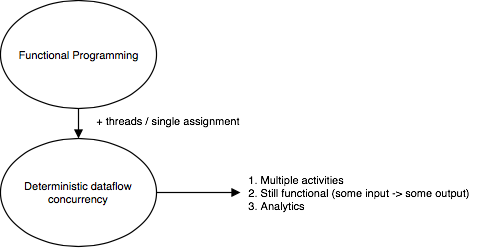
\includegraphics[width=0.83\textwidth]{img/DeterministicDataflowConcurrency}
	\caption{Le paradigme du \og deterministic dataflow concurrency \fg{}
	est une extension de la programmation fonctionnelle.}
\end{figure}
Dans le \emph{dataflow}, les activités concurrentes sont indépendantes
mais elles peuvent s'échanger de l'information.
Pour s'échanger l'information,
l'affectation unique nous permet d'attendre
jusqu'à ce que les données soient disponibles.
\begin{figure}[H]
	\centering
	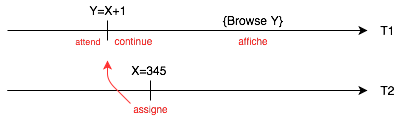
\includegraphics[width=0.83\textwidth]{img/MultipleThreads}
	\caption{Un exemple de synchronisation de dataflow:
	le premier thread doit attendre l'affectation dans le deuxième
	afin de pouvoir continuer.}
\end{figure}

Les \emph{threads} ne s'éxecutent pas en même temps.
L'ordre de l'exécution dépend de l'\emph{ordonnanceur} (\emph{scheduler}).
Voici un exemple d'exécution:
\begin{lstlisting}
declare A B C
thread A=1 end
thread B=2 end
thread C=A+B end
{Browse C}
\end{lstlisting}

Dans cet exemple, on crée 3 variables différentes,
ensuite 3 threads différents (on ne les exécute pas à ce moment-là),
et on fait l'appel à \lstinline|{Browse}|.

\begin{figure}[H]
	\centering
	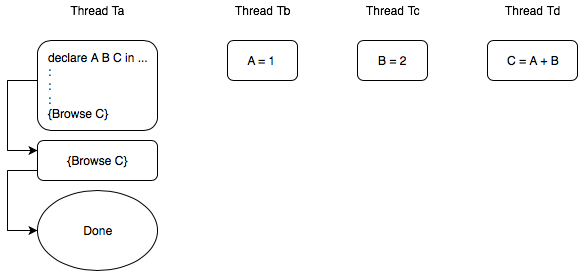
\includegraphics[width=0.83\textwidth]{img/ThreadVis}
	\caption{Visualisation des threads pour le programme précédent.
	L'appel à \lstinline[mathescape]|$\{$Browse$\}$| cache en fait
	la création d'un thread supplémentaire.}
\end{figure}

Les \emph{threads} sont indépendants et s'exécutent sur un même processeur,
qu'ils partagent en s'exécutant un par un.
Pour choisir l'ordre d'exécution des \emph{threads},
on utilise le \emph{scheduler}.
Les \emph{scheduler} a beaucoup de liberté
mais il doit avoir quelques propriétés:
\begin{itemize}
	\item \emph{équité}: il doit choisir chaque \emph{thread}
	qui est exécutable en un temps fini;
	\item \emph{intervalles de temps}: les \emph{threads}
	ont des petits intervalles d'exécution,
	en général $\approx \SI{10}{\milli\second}$;
	\item \emph{efficacité}:
	il ne doit pas prendre trop de temps pour faire ses choix.
\end{itemize}
Les \emph{threads} ont trois états:
\begin{itemize}
	\item \og \emph{completed}\fg;
	\item \og \emph{waits}\fg;
	\item \og \emph{time slice runs out}\fg.
\end{itemize}

Afin d'éviter le non-déterminisme lors de l'exécution du programme,
le paradigme a la propriété clef suivante:
\og \emph{le résultat de l'exécution ne dépend pas
de l'ordre dans lequel le scheduler choisit les threads,
et est donc le même pour tout choix fait par celui-ci}\fg.

\subsection{Programmation concurrente}
Pour faire de la programmation concurrente,
il faut savoir gérer les problèmes de synchronisation.

\begin{figure}[H]
	\centering
	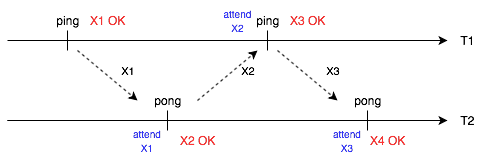
\includegraphics[width=0.83\textwidth]{img/PingPong}
	\caption{Un \emph{stream} est une liste avec une tail non affectée.}
\end{figure}

Une des techniques pour faire de la programmation concurrente
est d'utiliser des \emph{streams}
pour pouvoir communiquer entre les \emph{threads}.
\begin{mydef}
	Un \emph{stream} est une liste non bornée\footnote{C'est ici
	plus une intuition de parler de \og liste non bornée \fg,
	car une liste est toujours bornée par définition.} de messages
	où la tail est représentée
	par une variable \emph{dataflow} non affectée.
	Pour envoyer un message,
	on affecte à la fin de la liste un nouvel élément.
	Un \emph{agent} est un \emph{thread} qui utilise des \emph{streams}
	pour l'entrée/sortie.
\end{mydef}
Par exemple,
\begin{lstlisting}
declare Xs Xs2
Xs=0|1|2|3|4|Xs2
\end{lstlisting}

Le \emph{stream} est créé en affectant la tail
à une nouvelle liste avec une nouvelle tail:
\begin{lstlisting}
declare Xs3
Xs2=5|6|7|Xs3
\end{lstlisting}

\begin{mydef}
	On appelle \og\emph{producteur}\fg{}
	le \emph{thread} qui crée le \emph{stream}
	et \og\emph{consommateur}\fg{} le \emph{thread} qui le lit.
\end{mydef}
Voici un exemple d'un producteur-consommateur où on produit un \emph{stream}
et ensuite on calcule la somme de tous les élèments dans ce \emph{stream}:
\begin{lstlisting}
fun {Generate N Limit}
	if N<Limit then
		N|{Generate N+1 Limit}
	else nil end
end

fun {Sum Xs A}
	case Xs
	of X|Xr then {Sum Xr A+X}
	[] nil then A
	end
end
\end{lstlisting}

\begin{figure}[H]
	\centering
	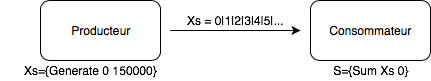
\includegraphics[width=0.83\textwidth]{img/ProdCons}
	\caption{Un schéma d'une relation producteur-consommateur.}
\end{figure}

Entre un \emph{producteur} et un \emph{consommateur},
on peut ajouter un filtre qui permettera de traiter
les données créés par le producteur
avant de les envoyer au consommateur.
\begin{myexem}
	\label{exem:prodcons}
	Par exemple, un producteur qui crée un \emph{stream},
	un \emph{filtre} qui ne laisse que les chiffres impairs
	et le \emph{consommateur} qui somme les élèments du \emph{stream}.
	\begin{figure}[H]
		\centering
		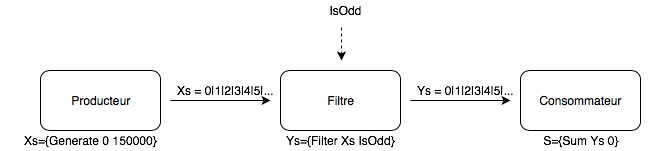
\includegraphics[width=0.83\textwidth]{img/ProdConsFilter}
		\caption{Un exemple de relation producteur-consommateur
		avec un filtre au milieu (Exemple~\ref{exem:prodcons}).}
	\end{figure}
\end{myexem}

\section{Concurrence déclarative}
Quand un programme contient des \emph{threads},
on ne sait pas prédire l'ordre d'exécution de ceux-ci.
Dans le cas où on a un seul \emph{thread},
\lstinline|thread| $\langle$s$\rangle$ \lstinline|end|,
l'exécution est séquentielle:
\begin{figure}[H]
	\centering
	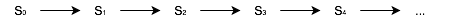
\includegraphics[width=0.5\textwidth]{img/SeqExec}
	\caption{Exemple d'exécution séquentielle.}
\end{figure}

Par contre, dès qu'on a plus d'un \emph{thread}, par exemple
\lstinline|thread| $\langle$s$\rangle_1$
\lstinline|thread| $\langle$s$\rangle_2$ \lstinline|end|
$\langle$s$\rangle_3$ \lstinline|end|,
l'exécution est un ordre partiel.
Cependant, sur un c\oe{}ur du processeur,
l'exécution est un ordre total grâce aux choix du \emph{scheduler}.
\begin{figure}[H]
	\centering
	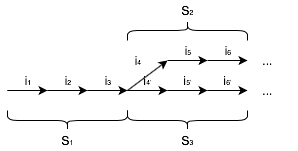
\includegraphics[width=0.5\textwidth]{img/ConcExec}
	\caption{Exemple d'exécution concurrente.}
\end{figure}
Dans ce cas, dès que l'instruction $\langle s \rangle_1$ est exécutée,
$\langle s \rangle_2$ et $\langle s \rangle_3$ commencent à s'exécuter
de façon concurrente.
\begin{figure}[H]
	\centering
	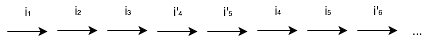
\includegraphics[width=0.5\textwidth]{img/ConcExecChoice}
	\caption{Un choix possible pour l'exécution concurrente
	(qui devient alors séquentielle).}
\end{figure}

L'exécution est appelée \emph{non détermininiste}
quand le système doit choisir lui-même l'ordre de l'exécution.
Le choix du \emph{thread} à exécuter est fait par un \emph{scheduler}.
À chaque pas de l'exécution, le \emph{scheduler}
doit choisir un des \emph{threads} qui sont prêts à s'exécuter.
Un \emph{thread} est prêt
s'il a toutes les informations pour exécuter une instruction.
Un \emph{thread} qui n'est pas prêt est appellé \og suspendu\fg.
Il ne peut pas continuer à s'exécuter parce qu'il n'a pas
assez d'informations pour pouvoir faire une étape de calcul.
On dit que sa première instruction est \og bloquée\fg.
On dit que le système est \emph{équitable}
si tous les \emph{threads}
dans l'état \og prêt\fg{} commencent à s'exécuter en temps fini.
Si un programme dans le paradigme \og deterministic dataflow\fg{}
est bien implémenté,
l'ordre de l'exécution ne peut pas influencer le résultat du programme
grâce à l'affectation unique.
En pratique, on utilise souvent différentes priorités
(\emph{high}, \emph{medium} ou \emph{low}),
pour aider l'ordonnanceur à répartir de façon optimale le temps d'exécution.

\begin{myexem}[Arbre d'exécution]
Le code suivant fait un simple calcul avec des \emph{threads}:
\begin{lstlisting}
thread A=1 end
thread B=2 end
thread C=A+B end
\end{lstlisting}
\begin{figure}[H]
	\centering
	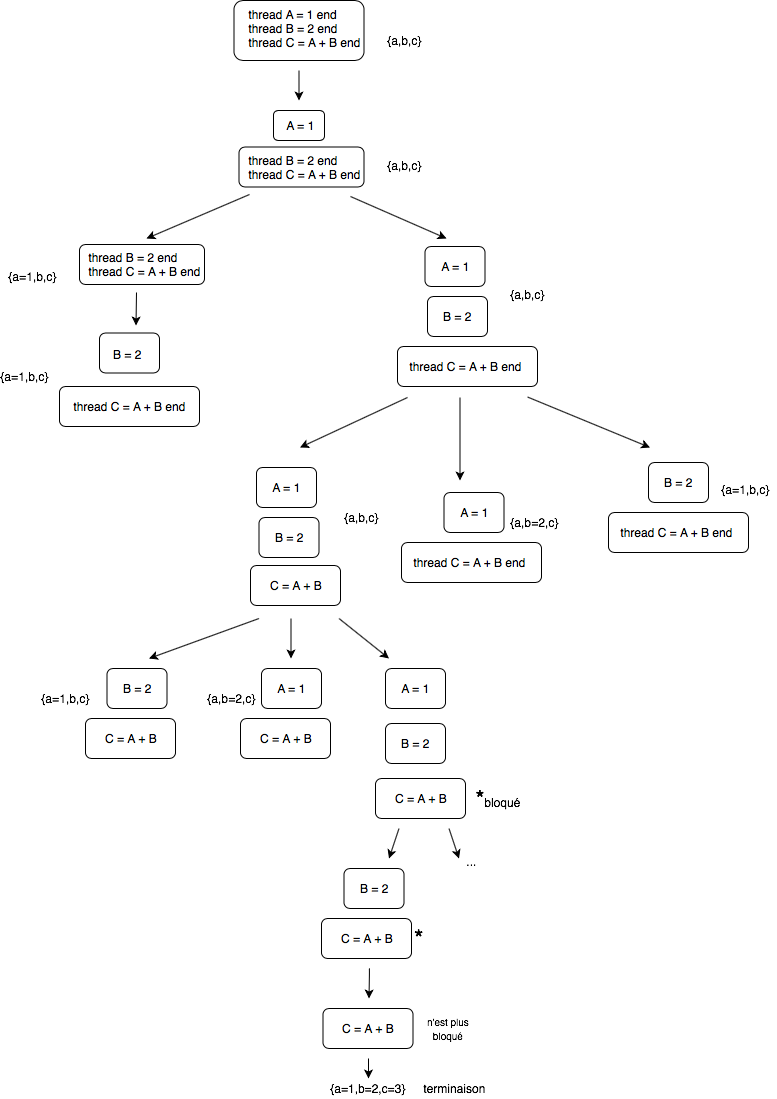
\includegraphics[width=0.7\textwidth]{img/ExecTree}
	\caption{Partie de l'arbre d'exécution complet
	pour le programme ci-dessus.}
\end{figure}
L'état final de l'exécution du programme
dans tous les cas est $\{a=1,b=2,c=3\}$.
\end{myexem}

On peut donc en quelque sorte considérer un thread comme une unité d'attente.
Dans le paradigme deterministic dataflow,
on peut ajouter autant de threads que l'on veut
sans influencer la correction du programme.

\section{Circuits logiques}
\subsection{Logique combinationnelle}
Définissons quelques connecteurs logiques qui sont souvent utilisés:
\begin{figure}[H]
\centering
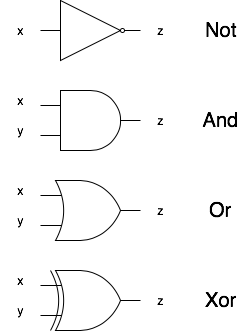
\includegraphics[width=0.4\textwidth]{img/LogicGates}
\caption{Représentations des portes logiques.}
\label{fig:logicgates}
\end{figure}

\lstinline|GateMaker| prend en argument un connecteur logique
et l'applique à deux \emph{streams}.
Il n'y a pas de mémoire.
\begin{lstlisting}
declare
fun {GateMaker F}
	fun {$ S1 S2}
		fun {GateLoop S1 S2}
			case S1|S2
			of (E1|T1)|(E2|T2) then {F E1 E2}|{GateLoop T1 T2} end
		end
	in
		thread {GateLoop S1 S2} end
	end
end

declare AndG OrG XorG in
AndG={GateMaker fun {$ A B} A*B end}
OrG={GateMaker fun {$ A B} X+Y-X*Y end}
XorG={GateMaker fun {$ A B} X+Y-2*X*Y end}
\end{lstlisting}

On peut également construire des circuits combinés.
Par exemple, un circuit combiné typique est le \emph{full adder},
qui somme trois nombres avec un seul bit
tel que le résultat est un nombre à deux bits.
Un full adder a trois \emph{inputs}: \(x\), \(y\), \(z\)
et deux \emph{outputs} \(c\) et \(s\),
tels que \(x + y + z = (cs)_2\).
\begin{figure}[H]
\centering
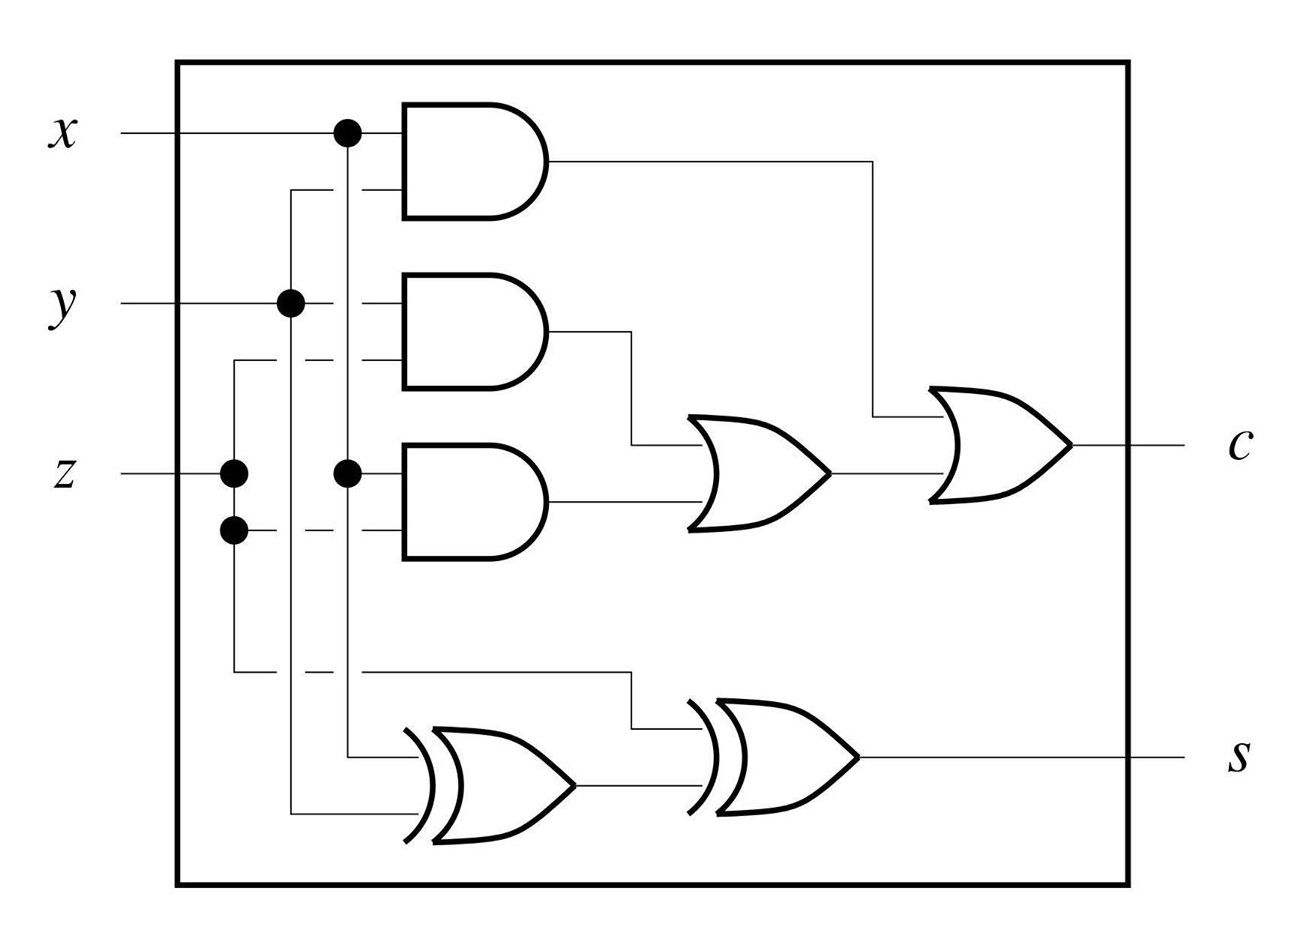
\includegraphics[width=0.6\textwidth]{img/FullAdder}
\caption{Vue schématique du \emph{full adder}.
On remarque qu'il faut sept threads, un pour chaque connecteur.}
\label{fig:fulladder}
\end{figure}

On peut définir \texttt{FullAdder} comme suit:
\begin{lstlisting}
declare
proc {FullAdder X Y Cin ?S ?Cout}
	A D E F G
in
	A={XorG Y Cin}
	S={XorG X A}
	D={AndG X Y}
	E={AndG X Cin}
	F={AndG Y Cin}
	G={OrG D E}
	Cout={OrG G F}
end
\end{lstlisting}

Il y a également moyen de concaténer les full adders
de sorte à créer un \emph{\(N\)-bit adder}
qui suit le même principe que le premier
sauf qu'il est utilisable pour les chaînes de bits.
\begin{figure}[H]
\centering
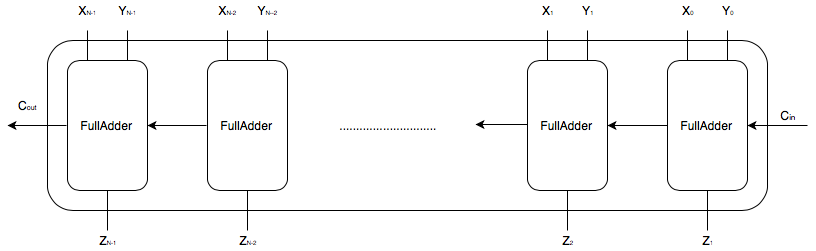
\includegraphics[width=0.6\textwidth]{img/NBitAdder}
\caption{Vue schématique du \emph{\(N\)-bit adder}.}
\label{fig:nbitadder}
\end{figure}

\begin{lstlisting}
declare
proc {NBitAdder Xs Ys Cin ?Zs ?Cout}
	case Xs|Ys
	of (X|Xr)|(Y|Yr) then Cm Z Zr in
		Zs=Z|Zr
		{FullAdder X Y Cm Z Cout}
		{NBitAdder Xr Yr Cin Zr Cm}
	[] nil|nil then % Zero-bit adder
		Zs=nil
		Cout=Cin
	end
end
\end{lstlisting}

\subsection{Logique séquentielle}
On peut aussi modéliser les circuits séquentiels.
Cela veut dire que certains \emph{outputs}
sont retournés comme \emph{inputs}.
Pour produire un \emph{output} nous avons besoin d'un \emph{input}.
Pour résoudre le problème de \emph{deadlock} qui peut se produire,
on va introduire une fonction \texttt{DelayG}
qui va gérer le délai en ajoutant un élement à la tête de la liste.

\begin{lstlisting}
fun {DelayG Xs}
	0|Xs
end
\end{lstlisting}

On va construire un exemple de \texttt{Latch}
qui mémorise son \emph{input} (ceci ne serait pas possible sans délais):
\begin{lstlisting}
fun {Latch C DI}
	DO X Y Z F
in
	F={DelayG DO}
	X={AndG F C}
	Z={NotG C}
	Y={AndG Z DI}
	DO={OrG X Y}
	DO
end
\end{lstlisting}
Un \emph{latch} a deux \emph{inputs}, \lstinline|C| et \lstinline|DI|.
On dit que \lstinline|C| est la \emph{clock}.
Si \lstinline|C| est à \(0\), alors l'\emph{output} va suivre \lstinline|DI|,
c'est-à-dire il aura la même valeur que \lstinline|DI|.
Si \lstinline|C| est égal à \(1\),
alors l'\emph{output} est \og gêlé \fg{}
sur la dernière valeur de \lstinline|DI| qu'il a suivie.
\begin{figure}[H]
\centering
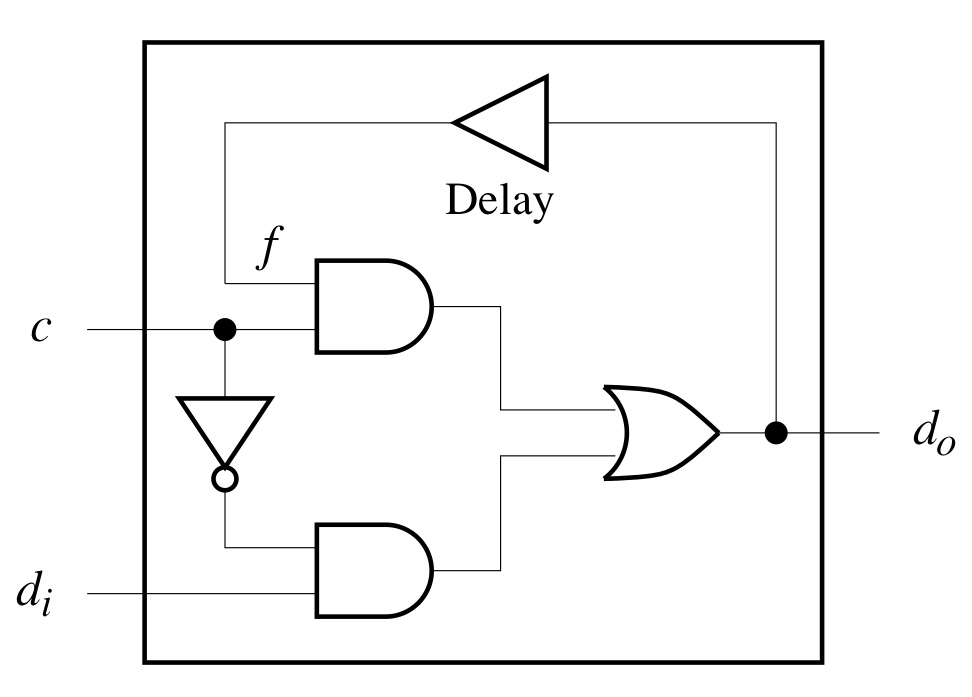
\includegraphics[width=0.6\textwidth]{img/Latch.jpg}
\caption{Représentation interne d'un \emph{latch}.
On remarque qu'il faut quatre threads,
un pour chaque connecteur mais pas pour le délai.}
\label{fig:latch}
\end{figure}
On peut écrire les équations logiques
pour le latch\footnote{Celles-ci peuvent changer
selon la définition de \emph{latch} qu'on utilise,
notamment quel état de la clock fait suivre l'output et quel état le gêle.}.
On commence par définir
\[
	\setlength{\tabcolsep}{0pt}
	\begin{array}{ccccccccccc}
	\texttt{DI} & = & d_0 & \mid & d_1 & \mid & \cdots & \mid & d_i & \mid & \cdots\\
	\texttt{C} & = & c_0 & \mid & c_1 & \mid & \cdots & \mid & c_i & \mid & \cdots\\
	\texttt{DO} & = & e_0 & \mid & e_1 & \mid & \cdots & \mid & e_i & \mid & \cdots
	\end{array}
\]
On peut alors écrire en regardant le circuit de la \figuref{latch} que
\begin{align*}
	e_i &= (c_i \overset{\textnormal{AND}}{\cdot} e_{i-1}) \overset{\textnormal{OR}}{+} (\overset{\textnormal{NOT}}{\overline{c_i}} \overset{\textnormal{AND}}{\cdot} d_i)\\
	\implies e_i &= \left\{
	\begin{array}{l@{\quad}l}
		(c_i \cdot e_{i-1}) + (\overline{c_i} \cdot d_i)\,, & \textnormal{pour \(i > 0\)}\,,\\
		\overline{c_0} \cdot d_0\,, & \textnormal{pour \(i = 0\)}\,.
	\end{array}
	\right.
\end{align*}
On trouve donc bien que si \(c_i = 1\), alors \(e_i = e_{i-1}\),
alors que si \(c_i = 0\), alors \(e_i = d_i\),
ce qui montre que le circuit fonctionne comme on veut.

\subsection{Exécution \og lazy \fg}
Pour pouvoir faire du \emph{dataflow},
nous avons besoin de deux fonctions:
\begin{itemize}
	\item \lstinline|{Wait X}|,
	qui attend jusqu'à ce que \lstinline|X| ait une valeur et
	\item \lstinline|{Bind X V}| qui affecte la valeur \lstinline|V|
	à la variable \lstinline|X|.
\end{itemize}

En introduisant une troisième fonction \lstinline|{WaitNeeded X}|,
qui arrête le thread courant
jusqu'à ce qu'un autre thread appelle \lstinline|{Wait X}|,
on peut faire de la programmation \og \lstinline|lazy|\fg,
avec le paradigme \emph{lazy deterministic dataflow}.
On peut introduire les fonctions \lstinline|lazy|.
Une instruction \lstinline|lazy| est donc exécutée
uniquement dans le cas où on a besoin de son résultat
quelque part dans le programme.

\begin{myexem}
\begin{lstlisting}
fun {F X}
	X*X
end
Y={F 10}
\end{lstlisting}
Le premier cas est basique, on affecte à \lstinline|Y|
le résultat de la fonction \lstinline|F|.
Donc \lstinline|Y| est directement affecté à la valeur \(100\).

\begin{lstlisting}
fun lazy {F X}
	X*X
end
Y={F 10}
{Browse Y+5}
\end{lstlisting}

Dans le cas de fonction \lstinline|lazy|,
à la quatrième ligne rien n'est affecté à \lstinline|Y|.
Pour calculer \lstinline|Y|,
on va attendre que le programme ait besoin de sa valeur.
Par exemple, à la cinquième ligne,
on aimerait bien afficher le résultat \lstinline|Y+5|.
C'est à ce moment-là que \lstinline|Y| est calculé
et que la valeur \(100\) lui est affectée.
\end{myexem}

Dans la langage noyau,
on a donc
\begin{lstlisting}[mathescape]
fun lazy {F X}
	$\langle$expr$\rangle$
end
\end{lstlisting}
qui devient
\begin{lstlisting}[mathescape]
proc {F X ?R}
	thread
		{WaitNeeded R}
		R=$\langle$expr$\rangle$
	end
end
\end{lstlisting}

\paragraph{Bounded buffer}
Un \emph{bounded buffer} est un buffer entre le producteur et le consommateur.
Il permet un juste milieu entre l'exécution \emph{eager} et \emph{lazy},
en stockant un certain nombre d'éléments produits non consommés.
Dans un programme \emph{eager}, la condition d'arrêt est dans le producteur,
alors que dans un programme \emph{lazy}, elle est dans le consommateur.

\section{Limitations du dataflow déterministe}
Les propriétés du dataflow déterministe sont:
\begin{itemize}
	\item la concurrence est facile,
	très similaire à la programmation fonctionnelle;
	\item le résultat est toujours le même,
	indépendamment du \emph{scheduler};
	\item grand potentiel du calcul.
\end{itemize}

\subsection{Client/serveur}
Par contre, pas tous les problèmes ne peuvent être correctement résolus
avec la concurrence \emph{dataflow}.
Par exemple, le problème de client/serveur
avec deux clients indépendants ne peut être résolu.
Le fait qu'ils soient indépendants implique qu'ils sont concurrents.
Vu qu'ils sont indépendants,
le serveur peut recevoir l'information des deux clients en même temps.
On va examiner ce problème plus profondément pour voir
pourquoi il n’est pas possible de le résoudre en \emph{dataflow} déterministe.

\begin{myexem}[Client/serveur]
\begin{figure}[H]
	\centering
	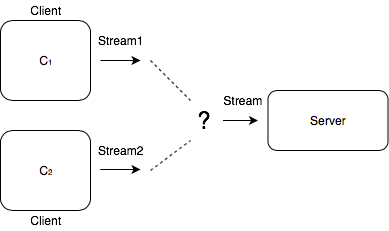
\includegraphics[width=0.7\textwidth]{img/cliservimposs}
	\caption{Le problème du client-serveur.}
\end{figure}
Le serveur a un flux d'entrée où il lit les commandes.
Supposons que le premier client envoie une commande au serveur.
Cela marche parfaitement, le serveur lit bien la commande.
Ensuite, le deuxième client veut se connecter au serveur,
donc il doit obtenir l'accès au flux pour se connecter au serveur.
Le problème est que ce flux n'existe pas;
il y a qu'un seul flux, entre le premier client et le serveur.
Le deuxième client ne peut pas s'approprier ce flux,
car cela posera des problèmes au premier client.

La première solution est de laisser au serveur deux flux d'entrée.
Mais dans ce cas, on ne sait pas déterminer l'ordre de préférence.
Supposons que l'information arrive des deux flux.
Alors est-ce qu'on lit toujours le premier d'abord, où le deuxième,
où un élément de chaque flux simultanément?
En effet, il n'y a pas de solution possible avec le \emph{dataflow}
parce que le dataflow suppose
que l'on connaisse l'ordre des requêtes des clients à l'avance.
Le problème du client/serveur est intrinsèquement non déterministe.
\end{myexem}

\subsection{\lstinline|WaitTwo|}
Pour décrire ce genre de programme,
une solution possible est d'ajouter une nouvelle opération \lstinline|WaitTwo|
qui attend l'information des deux clients en même temps:
\begin{lstlisting}
thread X = a end
thread Y = b end
thread Z = {WaitTwo X Y} end
\end{lstlisting}
Le résultat et l'ordre d'exécution dépendent du \emph{scheduler} et
est donc observablement non déterministe.
Le programme suivant résout le problème de deux clients et un serveur:
\begin{lstlisting}
proc{Server S1 S2}
	Z = {WaitTwo S1 S2}
in
	case Z|S1|S2
	of 1|(Q1|T1)|S2 then
		handle Q1
		{Server T1 S2}
	[] Z|S1|(Q2|T2) then
		handle Q2
		{Server S1 T2}
	end
end
\end{lstlisting}

Avec cette opération, le serveur sait attendre les commandes des deux clients.
Avec \lstinline|WaitTwo|, on pourrait bien résoudre le problème
même avec plus que deux clients,
mais la solution, qui paraît assez intuitive et facile,
est difficilement implémentable sur un ordinateur.
En effet, il faudrait traiter chaque ordre possible séparément,
ce qui donne lieu à un arbre de choix \lstinline|WaitTwo|.

\section{Message-passing concurrency}
La \emph{message-passing concurrency}
étend le modèle declaratif concurrent en ajoutant les \emph{ports}.
Il s'agit d'une autre façon d'ajouter du non-déterminisme dans un programme.
\begin{mydef}[Port]
	Les \emph{ports} sont les canaux de communication.
	Les ports ne sont pas déclaratifs
	car ils permettent des exécutions \emph{non déterministes}:
	beaucoup de \emph{threads} peuvent envoyer un message sur le port et
	leur ordre n'est pas contraint.
	Un port est un type abstrait de données avec deux opérations:
	\lstinline|{NewPort S P}| crée un nouveau port
	avec comme nom \lstinline|P| et lié au stream \lstinline|S|,
	alors que \lstinline|{Send P X}| envoie les informations à ce port,
	c'est-à-dire ajoute \lstinline|X| à la fin du stream
	qui correspond au port \lstinline|P|.
	Il s'agit d'objects actifs.
\end{mydef}

\subsection{Sémantique}
\subsubsection{\lstinline|NewPort|}
L'expression sémantique
\(\{\np\ \langle x \rangle\ \langle y \rangle\}, E)\)
fait les choses suivantes:
\begin{itemize}
	\item On crée un nouveau port nommé $n$.
	\item On lie \(E(\langle y \rangle)\) et $n$
	dans la mémoire à affectation unique.
	\item Si la liaison est réussie,
	on ajoute une paire \(E(\langle y \rangle):E(\langle x \rangle)\)
	dans la mémoire à affectation multiple.
	\item Si la liaison n'est pas réussie,
	alors une erreur est retournée.
\end{itemize}

\subsubsection{\lstinline|Send|}
L'expression sémantique
\(\{\send\ \langle x \rangle\ \langle y \rangle\}, E)\)
fait les choses suivantes:
\begin{itemize}
	\item Si la condition d'activation est vraie
	(\(E(\langle x \rangle\)) est déterminé), alors:
	\begin{itemize}
		\item Si \(E(\langle x \rangle)\) n'est pas attaché
		à un nom de port,
		alors une erreur est retournée.
		\item Si la mémoire à affectation multiple
		possède \(E(\langle x \rangle):z\), alors
		\begin{itemize}
			\item On crée une nouvelle variable $z'$ en mémoire.
			\item Ensuite, on met à jour
			la mémoire à affectation multiple:
			\(E(\langle x \rangle):z'\).
			\item Pour finir, on crée une nouvelle liste
			\(E(\langle y \rangle) \mid z'\)
			et on assigne sa valeur à $z$
			dans la mémoire à affectation unique.
		\end{itemize}
	\end{itemize}
	\item Sinon, l'exécution est suspendue.
\end{itemize}

\begin{figure}[!htbp]
	\centering
	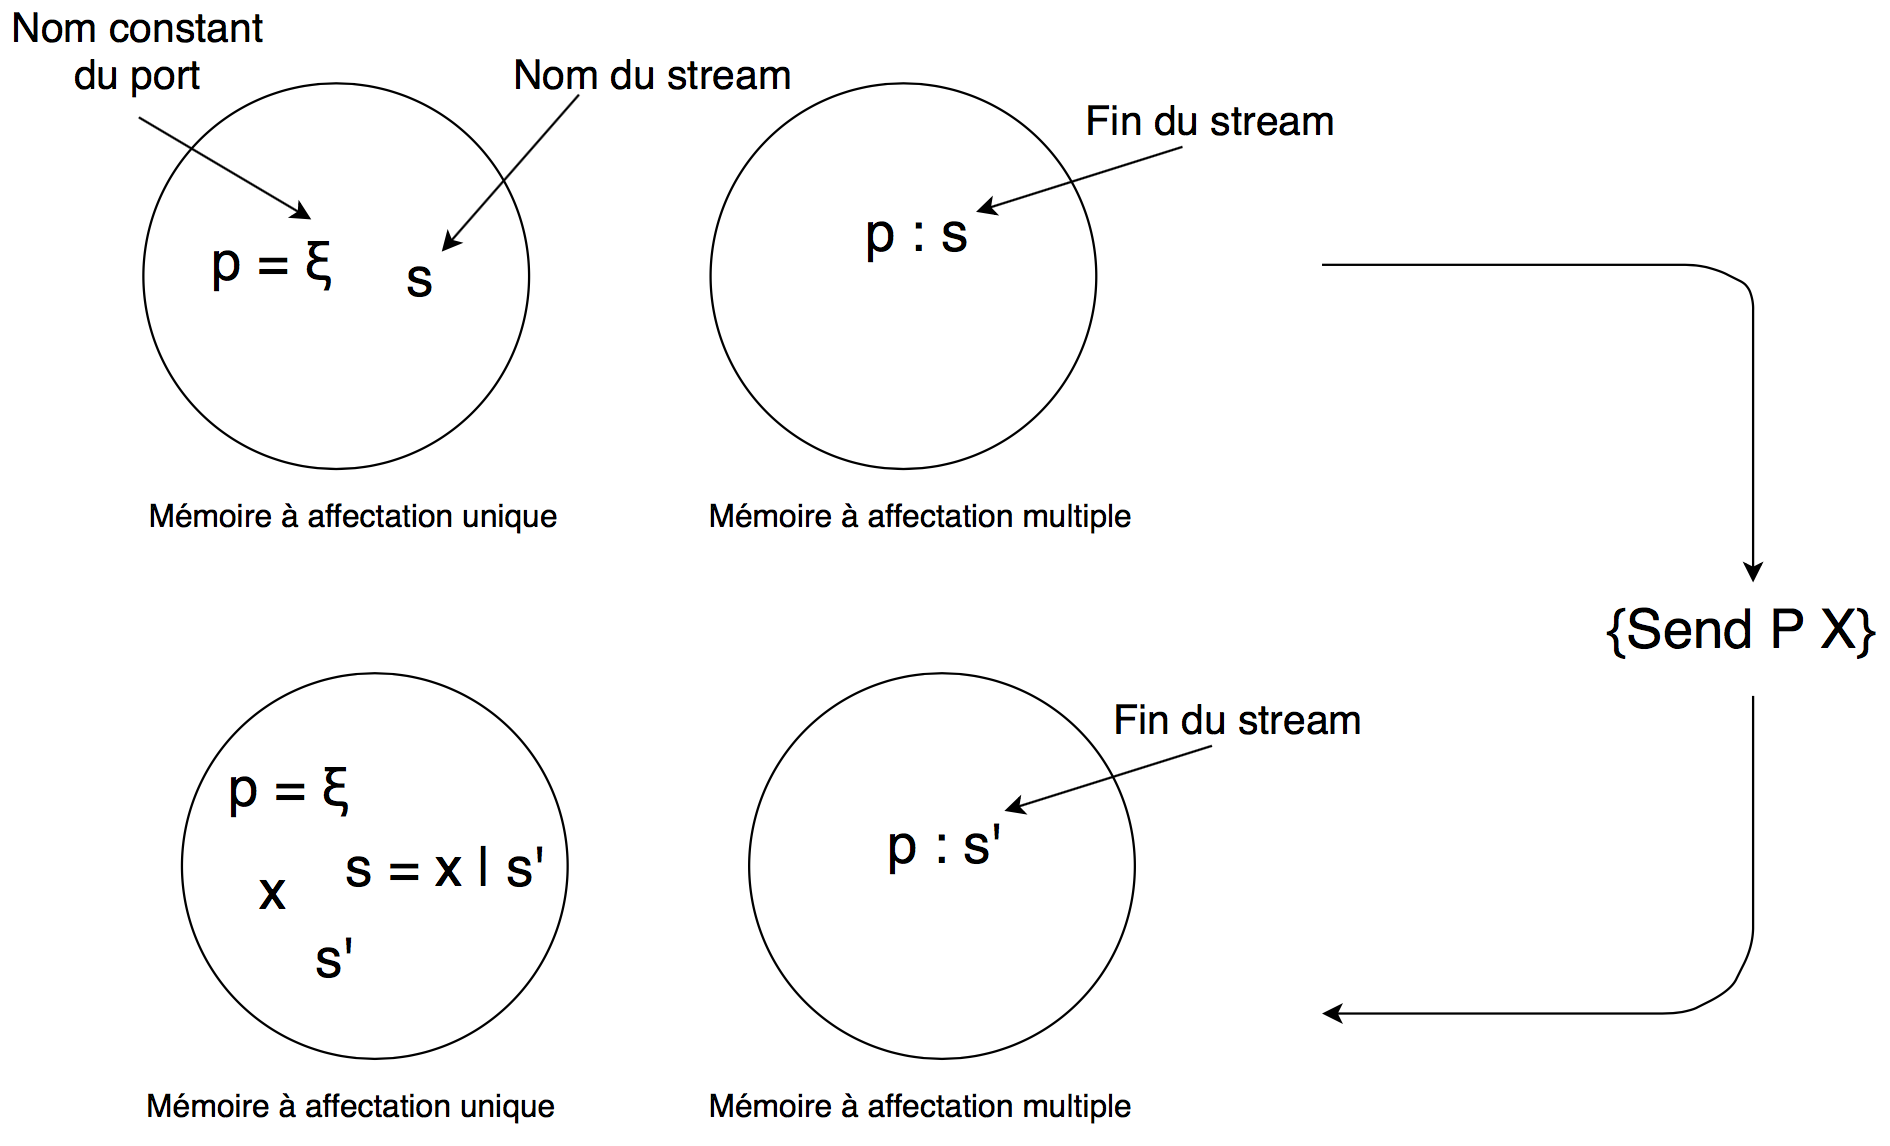
\includegraphics[width=0.7\textwidth]{img/sendmemory}
	\caption{L'évolution de la mémoire
	lors de l'opération \lstinline|Send|.}
\end{figure}

\subsection{Client-serveur}

\begin{figure}[!htbp]
	\centering
	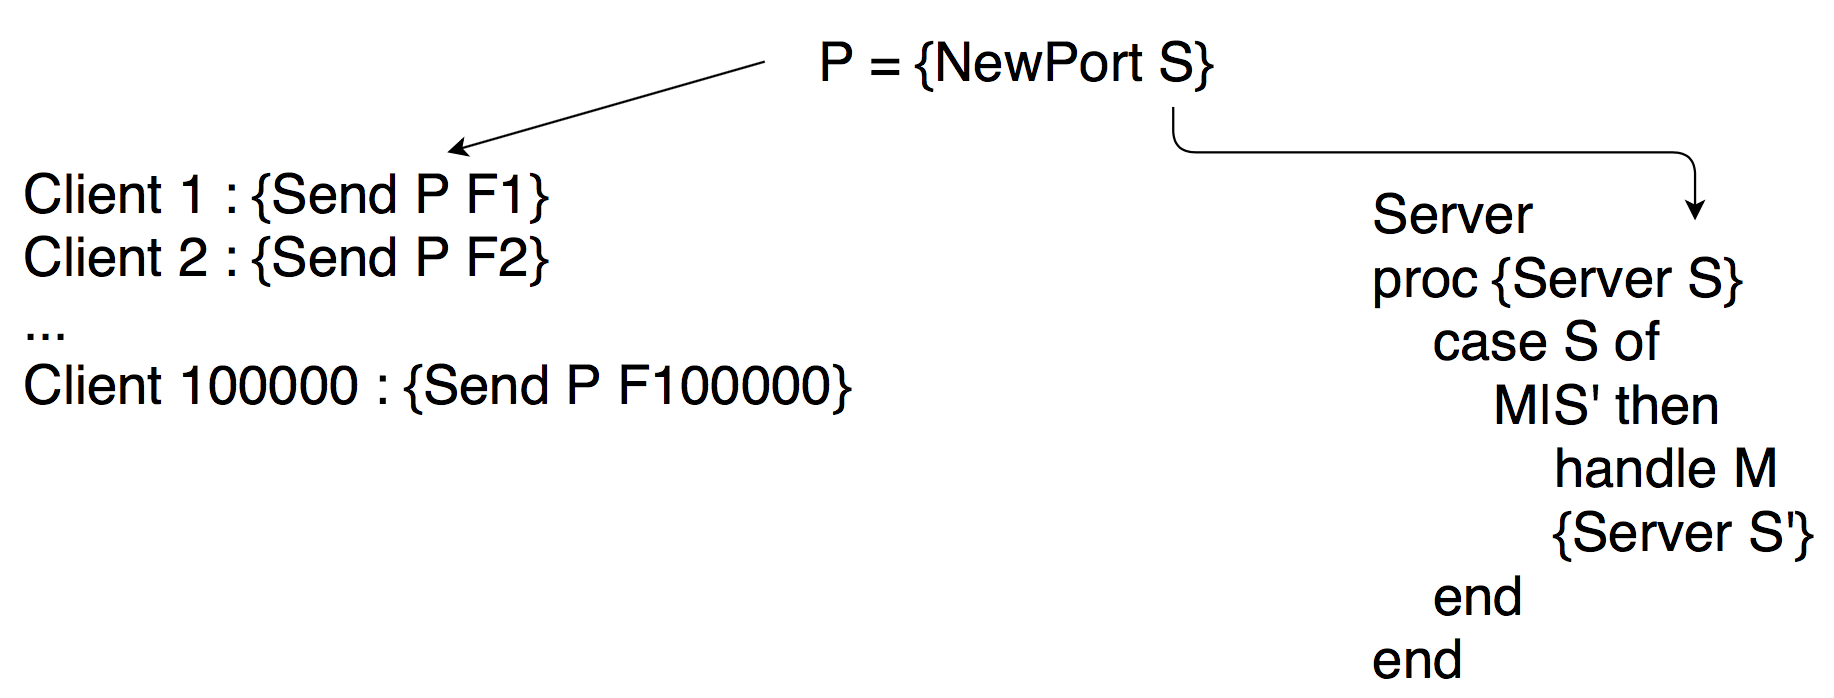
\includegraphics[width=0.7\textwidth]{img/cliserv}
	\caption{Code pour le problème client-serveur.}
\end{figure}

\begin{figure}[!htbp]
	\centering
	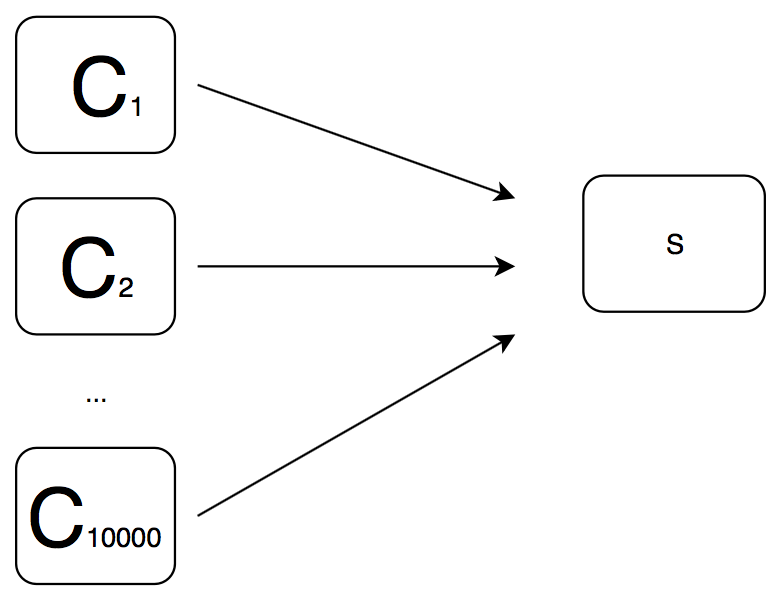
\includegraphics[width=0.7\textwidth]{img/cliserv2}
	\caption{La solution proposée s'adapte facilement
	à un nombre quelconque de clients.}
\end{figure}

\subsection{Objet port}
\begin{mydef}[Objet port]
	Un objet port est une combinaison d'un ou plusieurs ports et un stream.
	Ceci élargit le concept du simple stream
	parce que plusieurs threads peuvent envoyer de l'information
	sur le même port, indépendamment l'un de l'autre.
\end{mydef}

La structure d'un objet port est la suivante:
\begin{lstlisting}
declare P1 P2 ... Pn in
local S1 S2 ... Sn
	{NewPort S1 P1}
	{NewPort S2 P2}
	...
	{NewPort Sn Pn}
	thread {RP S1 S2 ... Sn} end
end
\end{lstlisting}
Ici, \lstinline|RP| est une fonction récursive
qui lit les streams de chaque port
et fait quelque chose pour chaque message reçu.

\begin{myexem}
	Trois joueurs sont dans un cercle et font passer un ballon entre eux.
	Quand un joueur attrape le ballon,
	il choisit un autre joueur au hasard et lui passe le ballon.
	Cette situation peut être modelisée avec des ports:
	\begin{figure}[!htbp]
		\centering
		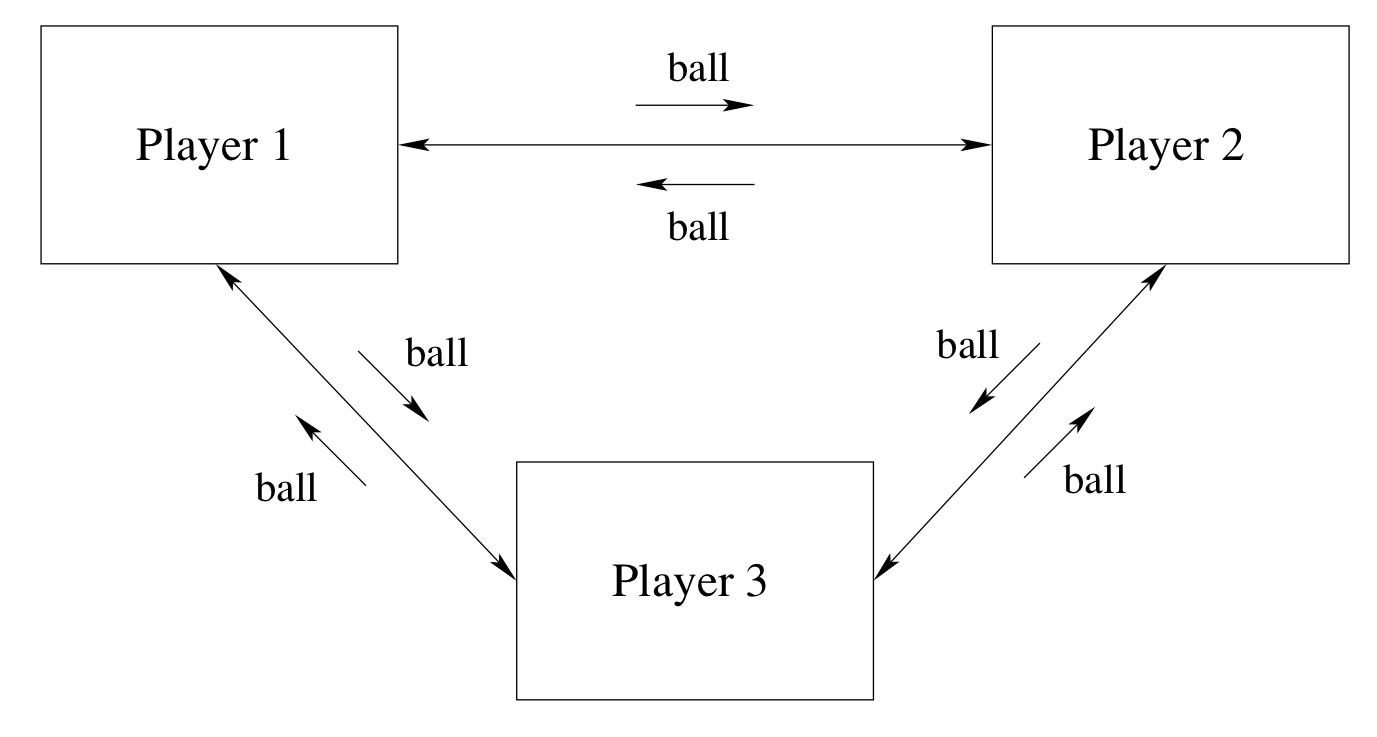
\includegraphics[scale = 0.5]{img/ballgame}
		\caption{Jeu avec le ballon.}
	\end{figure}

	La fonction suivante crée un nouveau joueur:
	\begin{lstlisting}
	fun {Player Others}
		{NewPortObject2
		proc {$ Msg}
			case Msg of ball then
				Ran = {Os.rand} mod {Width Others} + 1
			in
				{Send Others.Ran ball}
			end
		end}
	end
	\end{lstlisting}
	Pour commencer le jeu, on lance le ballon vers un des joueurs.
	\begin{lstlisting}
	P1 = {Player others(P2 P3)}
	P2 = {Player others(P1 P3)}
	P3 = {Player others(P2 P1)}

	{Send P1 ball}
	\end{lstlisting}
\end{myexem}

\subsection{Protocoles}
\begin{figure}[!htbp]
	\centering
	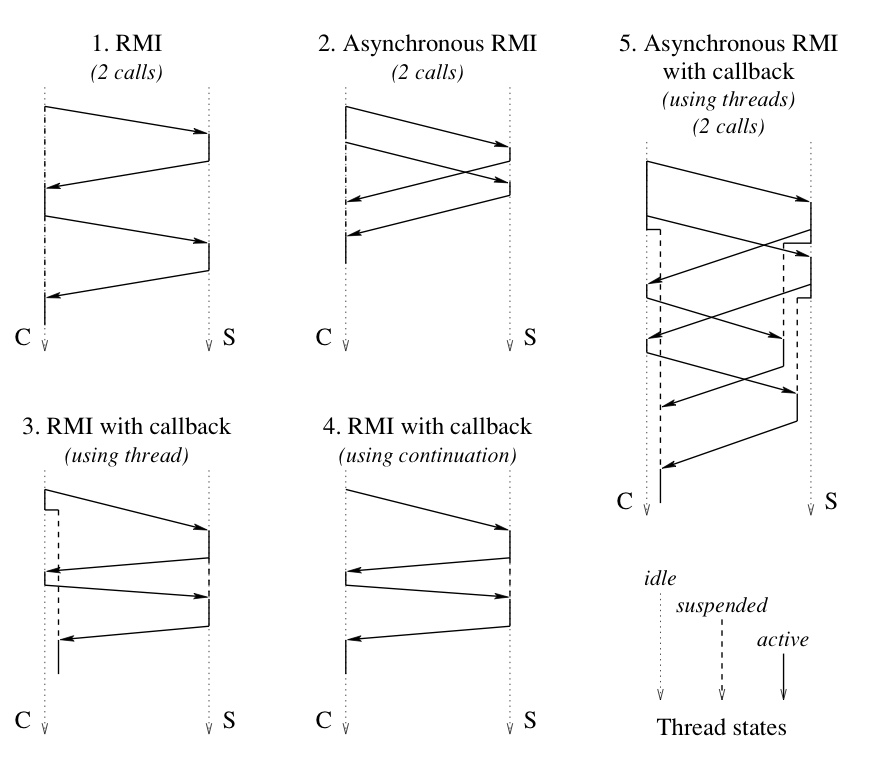
\includegraphics[scale = 0.7]{img/protocols}
	\caption{Protocoles de message simples.}
\end{figure}

\subsubsection{RMI (Remote Method Invocation)}
\label{sec:rmi}
\paragraph{Serveur}\leavevmode

\begin{lstlisting}
declare
proc {ServerProc Msg}
	case Msg
	of calc(X Y) then
		Y=X*X+123.0*X+34.4
	end
end
Server={NewPortObject2 ServerProc}

local Y in {Send Server calc(1.0 Y)} {Browse Y} end
\end{lstlisting}

\paragraph{Client}\leavevmode

\begin{lstlisting}
declare
proc {ClientProc Msg}
	case Msg
	of work(Y) then Y1 Y2 in
		{Send Server calc(10.0 Y1)}
		{Wait Y1}
		{Send Server calc(20.0 Y2)}
		{Wait Y2}
		Y=Y1+Y2
	end
end
Client={NewPortObject2 ClientProc}

local Y in {Send Client work(Y)} {Browse Y} end
\end{lstlisting}

\subsubsection{Asynchronous RMI}
\paragraph{Serveur}
Le serveur est le même que pour le protocole RMI en \sectionref{rmi},
et ne voit pas de différence en temps de calcul
entre ce protocole et le RMI simple.

\paragraph{Client}\leavevmode

\begin{lstlisting}
declare
proc {ClientProc Msg}
	case Msg
	of work(?Y) then Y1 Y2 in
		{Send Server calc(10.0 Y1)}
		{Send Server calc(20.0) Y2}
		Y = Y1 + Y2
	end
end
Client={NewPortObject2 ClientProc}

{Browse {Send Client work($)}}
\end{lstlisting}

\subsubsection{RMI with callback (avec des threads)}
\paragraph{Serveur}\leavevmode

\begin{lstlisting}
declare
proc {ServerProc Msg}
	case Msg
	of calc(X ?Y Client) then X1 D in
		{Send Client delta(D)}
		X1 = X+D
		Y = X1*X1+2.0*X1+2.0
	end
end

Server={NewPortObject2 ServerProc}
\end{lstlisting}

\paragraph{Client}\leavevmode

\begin{lstlisting}
declare
proc {ClientProc Msg}
	case Msg
	of work(?Z) then Y in
		{Send Server calc(10.0 Y Client)}
		thread Z = Y+100.0 end
	[] delta(?D) then
		D=1.0
	end
end

Client={NewPortObject2 ClientProc}
{Browse {Send Client work($)}}
\end{lstlisting}
Le thread est nécessaire, sinon on obtient un deadlock:
le client bloquerait sur cette opération,
et ne réagirait plus aux messages du serveur,
qui ne pourrait alors pas faire de callback.

\subsubsection{RMI with callback (avec la continuation des records)}
\label{sec:rmireccont}
\paragraph{Serveur}\leavevmode

\begin{lstlisting}
declare
proc {ServerProc Msg}
	case Msg
	of calc(X Client Cont) then X1 D Y in
		{Send Client delta(D)}
		X1 = X+D
		Y = X1*X1+2.0*X1+2.0
		{Send Client Cont#Y}
	end
end

Server={NewPortObject2 ServerProc}
\end{lstlisting}

\paragraph{Client}\leavevmode

\begin{lstlisting}
declare
proc {ClientProc Msg}
	case Msg
	of work(?Z) then
		{Send Server calc(10.0 Client cont(Z))}
	[] cont(Z)#Y then
		Z = Y+100.0
	[] delta(?D) then
		D=1.0
	end
end

Client={NewPortObject2 ClientProc}
{Browse {Send Client work($)}}
\end{lstlisting}

\subsubsection{RMI with callback (avec la continuation des procédures)}
\paragraph{Serveur}
Le serveur ne change pas par rapport à celui de la \sectionref{rmireccont}.

\paragraph{Client}\leavevmode

\begin{lstlisting}
declare
proc {ClientProc Msg}
	case Msg
	of work(?Z) then
		C = proc {$ Y} Z = Y+100.0 end
	in
		{Send Server calc(10.0 Client cont(C))}
	[] cont(C)#Y then
		{C Y}
	[] delta(?D) then
		D=1.0
	end
end

Client={NewPortObject2 ClientProc}
{Browse {Send Client work($)}}
\end{lstlisting}

\subsubsection{Asynchronous RMI with callback}
\paragraph{Serveur}\leavevmode
\begin{lstlisting}
declare
proc {ServerProc Msg}
	case Msg
	of calc(X ?Y Client) then X1 D in
		{Send Client delta(D)}
		thread
			X1 = X+D
			Y = X1*X1+2.0*X1+2.0
		end
	end
end

Server={NewPortObject2 ServerProc}
\end{lstlisting}

\paragraph{Client}\leavevmode

\begin{lstlisting}
declare
proc {ClientProc Msg}
	case Msg
	of work(?Y) then Y1 Y2 in
		{Send Server calc(10.0 Y1 Client)}
		{Send Server calc(20.0 Y2 Client)}
		thread Y = Y1 + Y2 end
	[] delta(?D) then
		D=1.0
	end
end

Client={NewPortObject2 ClientProc}
{Browse {Send Client work($)}}
\end{lstlisting}

\subsubsection{Double callbacks}
\paragraph{Serveur}\leavevmode
\begin{lstlisting}
declare
proc {ServerProc Msg}
	case Msg
	of calc(X ?Y Client) then X1 D in
		{Send Client delta(D)}
		thread
			X1 = X+D
			Y = X1*X1+2.0*X1+2.0
		end
	[] serverdelta(?S) then
		S = 0.01
	end
end

Server={NewPortObject2 ServerProc}
\end{lstlisting}

\paragraph{Client}\leavevmode

\begin{lstlisting}
declare
proc {ClientProc Msg}
	case Msg
	of work(Z) then
		{Send Server calc(10.0 Y Client)}
		thread Z = Y+100.0 end
	[] delta(?D) then S in
		{Send Server serverdelta(S)}
		thread D=1.0 end
	end
end

Client={NewPortObject2 ClientProc}
{Browse {Send Client work(Z)}}
\end{lstlisting}

Le thread chez le client est nécessaire car le client ne sait à priori pas
que le serveur va faire un autre callback.

\section{Multi-agent programming}
\subsection{Objets actifs et objets passifs}
\begin{table}[H]
	\centering
	\begin{tabular}{llll}
		\toprule
		Objets & Passif & Port & Actif\\
		\toprule
		Définition & Classe & Fonction de transition & Classe\\
		\midrule
		Exécution & Thread qui appelle & Propre thread & Propre thread\\
		\midrule
		Synchronisation & Synchronisé & Asynchronisé & Asynchronisé\\
		\midrule
		Méthodes & Pas d'ordre d'exécution & Exécutées séquentiellement & Exécutées séquentiellement\\
		\bottomrule
	\end{tabular}
	\caption{Comparaison entre les objets actifs, passifs et de port.}
\end{table}

\begin{myexem}[Classe \lstinline|PlayerClass| avec des objects actifs]
\begin{lstlisting}
declare
class PlayerClass
	attr state others
	meth init(Others)
		state := 0
		others := Others
	end
	meth ball
		Ran = ({OS.rand} mod {Width @others}) + 1
	in
		{(@others).Ran ball}
		state := @state + 1
	end
	meth get(X)
		X = @state
	end
end

declare
fun {Player Others}
	{NewActive PlayerClass init(Others)}
end

% Commencer la partie.
declare P1 P2 P3 in
P1 = {Player others(P2 P3)}
P2 = {Player others(P1 P3)}
P3 = {Player others(P1 P2)}

local X in {P1 get(X)} {Browse X} end
\end{lstlisting}
\end{myexem}

\subsection{Problème de Flavius Josephus}
Lorsque l'objet \(i\) reçoit le message \lstinline|kill(X S)|,
\begin{itemize}
	\item S'il est en vie et que $\texttt{S} = 1$,
	alors il est le dernier;
	on attache la variable globale à sa propre identité.
	\item S'il est en vie et $\texttt{S}>1$,
	alors si $\texttt{X} \mod k = 0$,
	il devient mort et envoie \lstinline|kill(X+1 S-1)| au suivant.
	\item S'il est en vie et \(\texttt{S} > 1\),
	alors si \(\texttt{X} \mod k \ne 0\),
	il envoie le message \lstinline|kill(X+1 S)| au suivant.
	\item S'il est mort, alors on envoie \lstinline|kill(X S)| au suivant.
\end{itemize}

\section{Component-based programming}
Le composant concurrent interagit avec l'environnement grâce à son interface.
L'interface contient un ensemble d'inputs et d'outputs,
qu'on appelle des \emph{wires}.
Un wire connecte un ou plusieurs outputs à un ou plusieurs inputs.
Il y a deux type de wire: one-shot et many-shot.
Le premier est implémenté avec des variables dataflow
et utilisé pour envoyer un seul message à la fois.
Seulement un message peut passer et seulement un output
peut être connecté à un input.
Le deuxième type, many-shot, est implémenté avec des ports.
Ici, plusieurs messages peuvent passer et plusieurs outputs
peuvent être connectés à un input.

\subsection{Les opérations basiques du component-based programming}
Il y a quatre opérations basiques:
\begin{description}
	\item[Instanciation]
	Création des instances d'un composant.
	Par défaut, chaque instance est indépendante
	des autres instances créés.
	\item[Composition]
	Construction d'un nouveau composant.
	Par défaut, les composants sont indépendants.
	\item[Mise en relation]
	Combiner les composants en connectant les outputs et les inputs.
	\item[Restriction]
	Limiter la visibilité des inputs et/ou des outputs
	à l'intérieur d'un composant.
\end{description}
L'exemple du latch montre comment modéliser les circuits avec les composants:
\begin{lstlisting}
proc {Latch C DI ?DO}
	X Y Z F
in
	{DelayG DO F}
	{AndG F C X}
	{NotG C Z}
	{AndF Z DI Y}
	{OrG X Y DO}
end
\end{lstlisting}
Dans cet exemple on observe la liaison des inputs et des outputs.
Par exemple, l'output \lstinline|X| du premier \lstinline|AndG|
est par après passé comme input à \lstinline|OrG|.

\subsection{Methodologie de conception}
Vu que dans la programmation concurrente, les différentes parties du programme
peuvent interagir entre elles,
on doit suivre des certaines règles pour avoir un programme correct:
\begin{itemize}
	\item Spécification informelle:
	écrire les spécifications précises
	de tout ce que le système doit faire.
	\item Composants: définir les composants, grâce à un schéma-bloc.
	\item Protocoles de message:
	décider comment les composants vont interagir entre eux.
	\item Diagramme d'état:
	pour chaque entité concurrente, écrire son état.
	\item Implémenter et ordonnancer:
	coder le système et décider l'algotithme d'ordonnancement utilisé
	pour implémenter la concurrence entre les composants.
	\item Tester et itérer: tester le système et itérer
	jusqu'à ce qu'il satisfasse les spécifications de base.
\end{itemize}

\subsection{Système de contrôle d'ascenseur}
On va faire le design du système de contrôle d'un ascenseur
en utilisant la méthodologie décrite ci-dessus.
\begin{figure}[H]
	\centering
	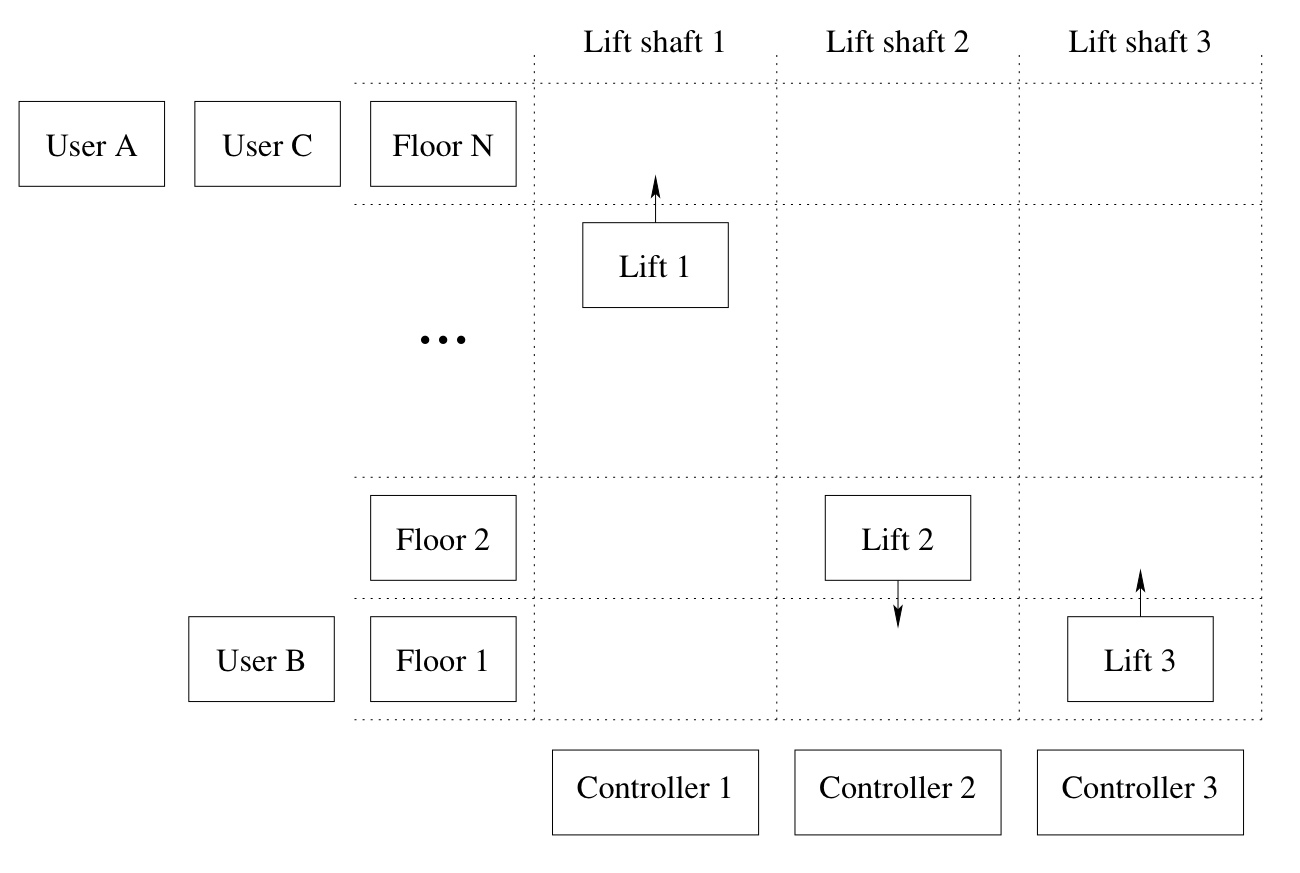
\includegraphics[width=\textwidth]{img/lift}
	\caption{Vue schématique d'un bâtiment avec des ascenseurs.}
\end{figure}

On commence par les spécifications.
On a un ensemble d'étages et un ensemble d'ascenseurs.
Chaque étage possède un bouton sur lequel l'utilisateur peut appuyer
et donc appeler l'ascenseur.
Le bouton ne spécifie pas la direction.
L'étage choisit de manière aléatoire quel ascenseur appeler.
Chaque ascenseur a un ensemble de boutons \lstinline|call(I)|
pour chaque étage \lstinline|I|
qui servent à dire qu'il doit s'arrêter à l'étage donné.
Chaque ascenseur a un ordonnanceur où on trouve
une liste des étages à visiter dans un certain ordre.
On va utiliser un algorithme FIFO pour ce système.

Pour faire le diagramme des composants,
on identifie qu'il y a en tout 4 composants:
des étages, des ascenseurs, des controllers et des timers.
Toutes les instances sont des objets ports.
Le controller est utilisé pour gérer les mouvements des ascenseurs.
Les timers sont là pour gérer l'aspect temps-réel du système:
\begin{figure}[H]
	\centering
	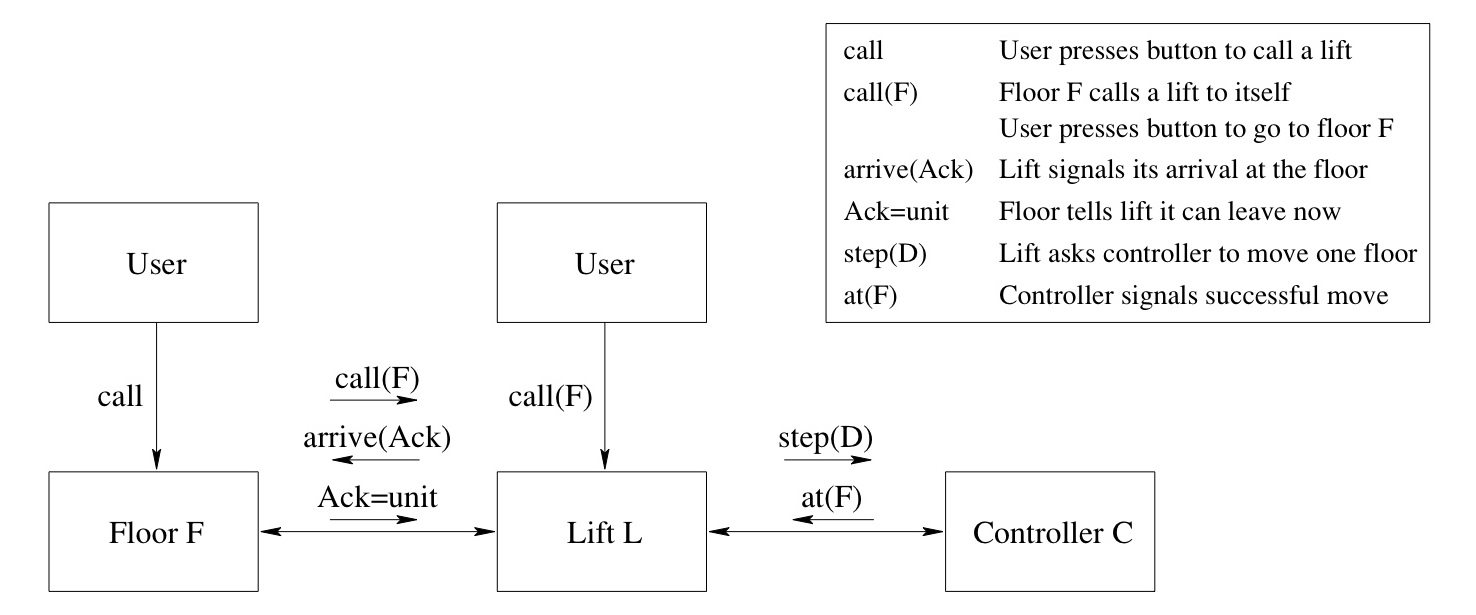
\includegraphics[width=0.7\textwidth]{img/componentDiag}
	\caption{Diagramme des composants du système de contrôle d'ascenseur.}
\end{figure}

Le controller a 2 états: motor stop et motor running.
Pour le premier état, le controller
peut recevoir un message \lstinline|step(Dest)| d'un ascenseur,
où \lstinline|Dest| est le numéro de l'étage.
En fonction de la direction,
le controller va bouger l'ascenseur en haut ou en bas.
Le controller utilise un timer
pour passer de l'état \emph{running} à l'état \emph{stop}:
\begin{figure}[H]
	\centering
	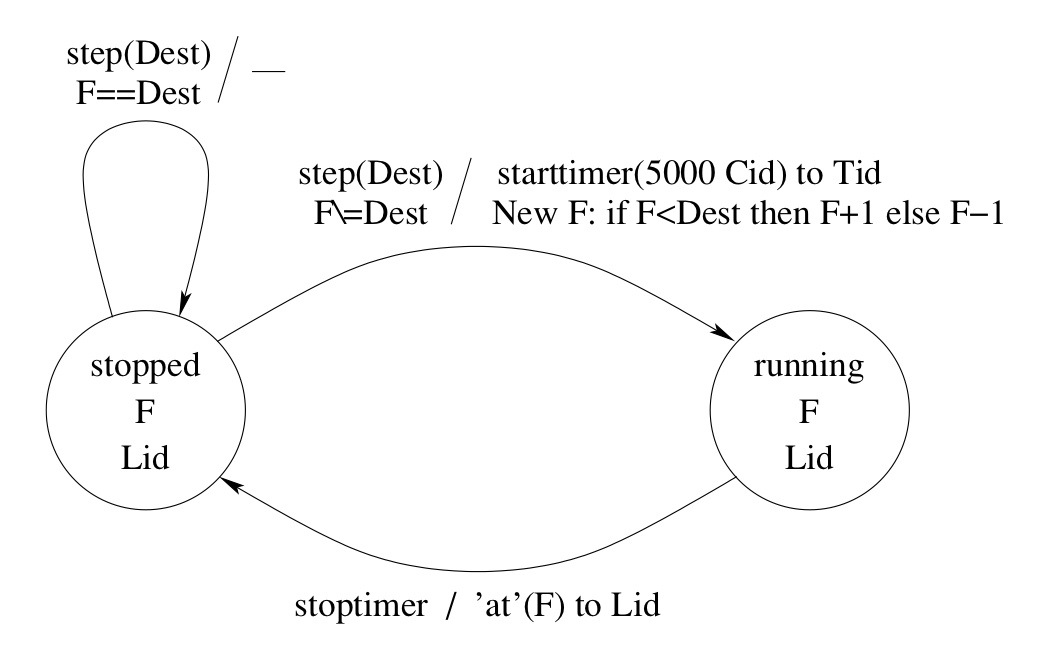
\includegraphics[width = 0.6\textwidth]{img/controller}
	\caption{Diagramme d'état du controller.}
\end{figure}

L'étage possède 3 états:
\begin{itemize}
	\item on a appelé un ascenseur et celui-ci arrive;
	\item on a appelé un ascenseur et les portes sont ouvertes et
	\item on n'a pas appelé d'ascenseur.
\end{itemize}
Chaque étage peut recevoir un message \lstinline|call| de l'utilisateur,
un message \lstinline|arrive(Ack)| de l'ascenseur et les messages du timer.
Aussi, l'étage peut envoyer un message \lstinline|call(F)| à l'ascenseur.
\begin{figure}[H]
	\centering
	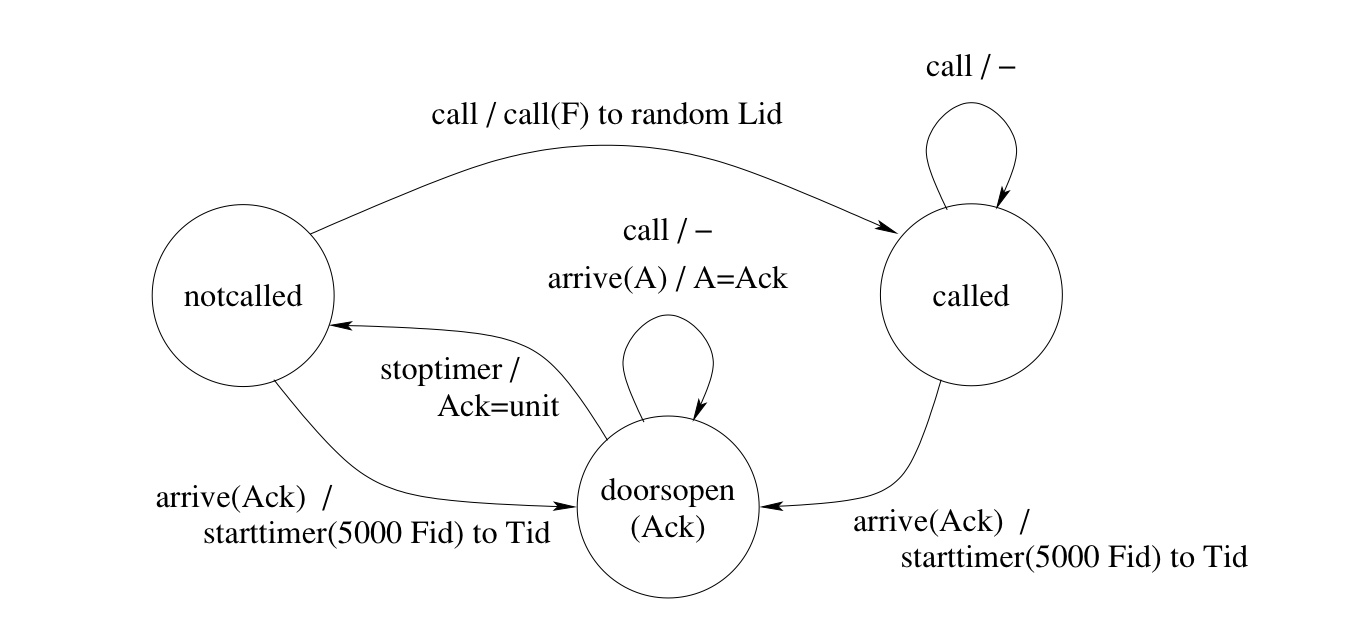
\includegraphics[width=0.6\textwidth]{img/Etage}
	\caption{Diagramme d'état d'un étage.}
\end{figure}

L'ascenseur possède 4 états:
\begin{itemize}
	\item pas d'appel et l'ascenseur est arrêté;
	\item il y a un appel et l'ascenseur bouge vers l'étage donné;
	\item attend que les portes s'ouvrent
	pour que quelqu'un sorte de l'ascenseur et
	\item attend que les portes s'ouvrent
	pour que quelqu'un entre dans l'ascenseur.
\end{itemize}
Chaque ascenseur peut recevoir un message \lstinline|call(N)|
et un message \lstinline|at(N)|.
L'ascenseur peut envoyer un message \lstinline|arrive(Ack)| à un étage
et un message \lstinline|step(Dest)| au controller.
Après avoir envoyé un message \lstinline|arrive(Ack)|,
l'ascenseur attend jusqu'à ce que l'étage lui envoie
une confirmation de la fermeture des portes.
\begin{figure}[H]
	\centering
	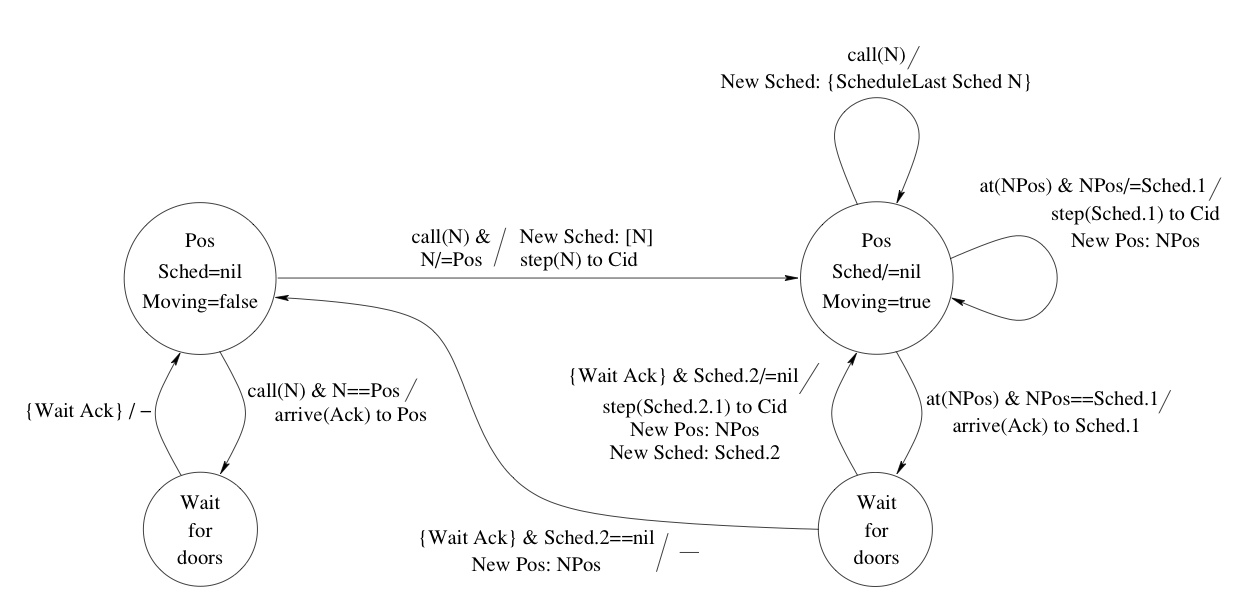
\includegraphics[width=0.7\textwidth]{img/LiftDiag}
	\caption{Diagramme d'état d'un ascenseur.}
\end{figure}

\section{Shared-state concurrency}
\subsection{Rappel}
Voici les opérations atomiques possibles:
\begin{itemize}
	\item \lstinline|C = {NewCell X}| crée une nouvelle cellule.
	\item \lstinline|C := X| assigne une valeur à une cellule.
	\item \lstinline|@C| lit la valeur de la cellule;
	par exemple: \lstinline|Y = @C + 1|.
	\item \lstinline|{Exchange C X Y}| change la valeur de la cellule
\end{itemize}

\begin{figure}[H]
	\centering
	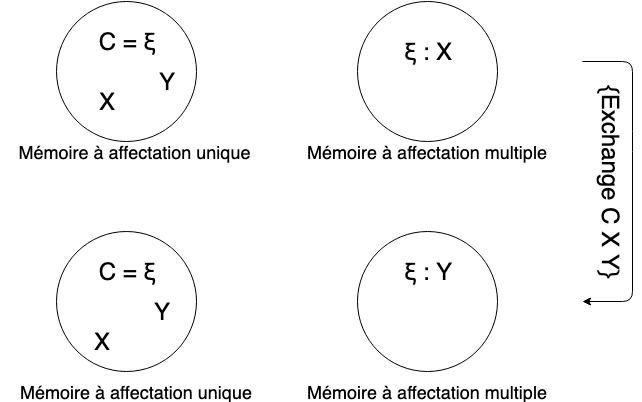
\includegraphics[width=0.7\textwidth]{img/cellsemantics}
	\caption{Sémantique des cellules.}
\end{figure}

Vu que les cellules peuvent changer de valeur,
la programmation avec les threads devient compliquée.
Pour mettre des règles sur qui et quand peut avoir accès à la cellule
et éventuellement changer sa valeur, on va introduire les \emph{locks}.
Les locks peuvent être de deux types: \emph{monitors} et \emph{transactions}.

\subsection{Locks}
Les locks utilisent la technique du token-passing
pour extraire un ordre d'exécution d'une part du programme
et l'imposer à une autre.
Le token-passing est implémenté
en créant une séquences de variables dataflow $X_0, X_1, X_2, \ldots$
et en passant les paires $(X_0, X_1), (X_1,X_2), \ldots$
aux opérations qui doivent être faites dans un certain ordre.
Une opération qui reçoit la paire $(X_i, X_{i+1})$
fait les choses suivantes:
\begin{itemize}
	\item elle attend jusqu'à ce que le token arrive,
	donc que $X_i$ soit attaché (\lstinline|{Wait Xi}|);
	\item elle fait ses calculs;
	\item elle envoie un token à la paire suivante,
	donc attache $X_{i+i}$.
\end{itemize}

\begin{figure}[H]
	\centering
	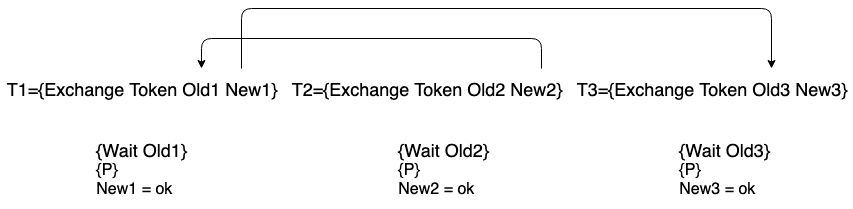
\includegraphics[width=\textwidth]{img/tokenpassing}
	\caption{Le thread \lstinline|T2| est exécuté en premier.
	Dès qu'il termine son exécution,
	il assigne la nouvelle valeur de la cellule
	à son argument \lstinline|New2|.
	Ensuite, le thread \lstinline|T1| est exécuté,
	avec comme ancienne valeur de \lstinline|Old1|, \lstinline|New2|.
	Le thread \lstinline|T3| fait pareil:
	il prend l'ancienne valeur de la cellule,
	c'est-à-dire la nouvelle valeur retournée par \lstinline|T1|,
	et il change encore sa valeur.}
\end{figure}

\begin{myexem}[File avec des locks]
Voici une implémentation d'un file concurrente et orientée-objet,
avec des locks.
\begin{lstlisting}
class Queue
	attr queue
	prop locking

	meth init
		queue := q(0 X X)
	end

	meth insert(X)
		lock N S E1 in
			q(N S X|E1) = @queue
			queue := q(N+1 S E1)
		end
	end

	math delete(X)
		lock N S1 E in
			q(N X|S1 E) = @queue
			queue := q(N-1 S1 E)
		end
	end
end
\end{lstlisting}
\end{myexem}

\subsubsection{Reentrant lock}
Le type de lock que nous utilisons est dit \og reentrant\fg{},
car il permet à un même thread de rentrer dans plusieurs zones critiques
protégées par un même lock.
Pour faire ceci, il faut donner un ID unique à chaque thread.

\subsection{Monitors}
Les locks sont importants pour faire de la programmation concurrente
mais ils ne savent pas faire tout.
Par exemple, si un thread veut accéder à un buffer pour y ajouter un élément,
il n’est pas suffisant de juste protéger le buffer avec un lock
car si le lock laisse entrer le thread et que le buffer est rempli,
il ne sait rien faire.
Nous avons donc besoin d’une structure qui va faire attendre le thread
jusqu'au moment qu'il y a une place libre dans le buffer;
ceci est possible en utilisant les \emph{monitors}.

Il y a 3 opérations pour gérer les monitors: \lstinline|wait|,
\lstinline|notify| et \lstinline|notifyAll|.
Ces opérations peuvent être appelées que par le thread qui tient le lock.

L'opération \lstinline|wait| fait les choses suivantes:
\begin{itemize}
	\item le thread courant est suspendu;
	\item le thread est placé dans l'ensemble d'attente interne de l'objet;
	\item le lock pour cet objet est libéré.
\end{itemize}

L'opération \lstinline|notify| fait les choses suivantes:
\begin{itemize}
	\item si l'ensemble d'attente interne de l'objet n'est pas vide,
	alors un thread \lstinline|T| y appartenant est choisi aléatoirement.
	\item \lstinline|T| rentre dans le lock.
	Il va être suspendu pour encore un peu de temps
	tant que le thread de notification ne libère pas le lock.
	\item \lstinline|T| reprend son exécution là où il a été suspendu.
\end{itemize}

L'opération \lstinline|notifyAll| est semblable à \lstinline|notify|,
sauf qu'elle fait toutes les opérations décrites ci-dessus
pour tous les threads dans l'ensemble d'attente interne de l'objet.

\begin{myexem}[Bounded buffer implémenté avec des monitors]\leavevmode
\begin{lstlisting}
declare
class Buffer
	attr m buf first last n i

	meth init(N)
		m:={NewMonitor}
		buf:={NewArray 0 N-1 null}
		n:=N i:=0 first:=0 last:=0
	end

	meth put(X)
		{@m.'lock' proc {$}
			if @i>=@n then
				{@m.wait} {self put(X)}
			else
			@buf.@last:=X
			last:=(@last+1) mod @n
			i:=@i+1
			{@m.notifyAll}
			end
		end}
	end

	meth get(X)
		{@m.'lock' proc{$}
			if @i==0 then {@m.wait} {self get(X)}
			else
				X=@buf.@first
				first:=(@first+1) mod @n
				i:=@i-1
				{@m.notifyAll}
			end
		end}
	end
end
\end{lstlisting}
\end{myexem}

\subsection{Transactions}
\begin{figure}[H]
	\centering
	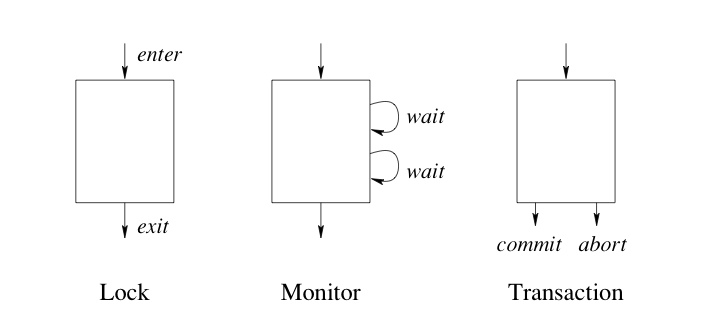
\includegraphics[width=\textwidth]{img/locks}
	\caption{Différences entre les actions atomiques.}
\end{figure}
Les transactions sont introduites pour résoudre
le problème des clients qui veulent mettre à jour
la base des données tous en même temps.
Dans ce cas, utiliser les locks n'est pas pratique,
car quand un client accède à la base des données,
il va bloquer tous les autres utilisateurs
et le processus sera inefficace.

Une transaction est une opération qui satisfait les 4 propriétés ACID:
\begin{itemize}
	\item Atomicité: on n'observe pas d'état intermédiaire
	de la transaction.
	Soit tout se fait instantanément, soit rien ne se fait.
	La transaction peut bien se terminer ou elle peut être annulée.
	\item Consistence: les changements respectent les invariants du système.
	\item Isolation: plusieurs transactions peuvent se produire
	sans qu'une puisse interférer avec une autre.
	\item Durabilité: les changements observables sont sauvegardés
	même si le système tombe en panne.
\end{itemize}

\subsubsection{Motivation}
La première raison pour introduire les transactions
est d'augmenter le nombre d'accès concurrents à la base des données.
La deuxième raison est de rendre possible
la programmation concurrente avec exceptions.
Les routines ont deux manières de se terminer:
soit elles se terminement normalement, soit il se produit une exception.
Quand elles se terminent normalement,
on ne voit que l'état initial et et l'état final, sans états intermédiaires.
Par contre, quand il y a une exception, nous avons deux solutions:
\begin{itemize}
	\item On \og nettoie\fg{} tout le désordre provoqué par la routine.
	Cette solution est simple à implémenter,
	mais la routine doit bien être écrite,
	sinon les dégâts peuvent être énormes.
	\item On met la routine dans une transaction.
	Cette solution est plus difficile à implémenter
	mais le programme devient plus simple.
	Si une exception apparaît, on annule la transaction.
\end{itemize}

\subsection{Two-phase locking}
Two-phasing locking est le système le plus populaire pour faire un lock.
La transaction a deux phases:
\begin{itemize}
	\item la phase de croissance, où elle acquiert un lock
	mais ne le libère pas;
	\item la phase de rétrécissement,
	où elle libère le lock mais ne l'acquiert pas.
\end{itemize}
La transaction n'a pas le droit de libérer un lock et
ensuite d'en acquérir un autre directement après.
Cela veut dire que la transaction peut contrôler un lock
pendant plus longtemps qu'elle n'en ait besoin.
On peut alors avoir un problème dit \og d'abort en cascade\fg{}.
Supposons qu'un thread \lstinline|T1|
accède à la cellule \lstinline|C| et la change.
Ensuite, \lstinline|T1| libère la cellule dans sa phase de rétrécissement
mais il reste toujours actif.
\lstinline|T2| accède alors à la cellule et la change.
Si maintenant \lstinline|T1| s'annule,
alors on doit aussi annuler \lstinline|T2| et
toutes les autres opérations qui ont été produites
avec la cellule en attendant.
Ce n’est pas pratique, du coup on utilise le \og strict two-phase locking\fg{}
où la cellule est libérée uniquement
lorsque la transaction est complétement finie ou annulée.

\subsection{Design du système de transactions}
L'algorithme naïf consiste à toujours donner un lock pour une cellule ouverte
à une transaction qui le demande.
Si la cellule est fermée, alors on laisse la transaction attendre
jusqu'à ce que la cellule s'ouvre.
Si la transaction est annulée, alors on libère tous les locks qu'elle possède.
L'algorithme est optimiste car il suppose
qu’avoir un lock ne peut pas poser de problèmes.
Si des problèmes se posent, alors l'algorithme doit les résoudre.

L'algorithme naïf peut produire des deadlocks.
Supposons que deux transactions \lstinline|T1| et \lstinline|T2|
veulent chacun accéder aux cellules \lstinline|C1| et \lstinline|C2|.
\lstinline|T1| utilise \lstinline|C1| puis \lstinline|C2|
et \lstinline|T2| utilise \lstinline|C2| puis \lstinline|C1|.
À cause de la concurrence, \lstinline|T1| bloque \lstinline|C1| et
\lstinline|T2| bloque \lstinline|C2|.
Quand ils essayent d'avoir le lock suivant,
donc \lstinline|T1| veut \lstinline|C2| et \lstinline|T2| veut \lstinline|C1|,
ils vont s'attendre indéfiniment l'un l'autre.
Il y a deux solutions à cela: une pessimiste et une optimiste.
La solution pessimiste va prévoir les deadlocks;
s’il y a une possibilité de deadlock,
on interdit à la transaction de lock une cellule.
La solution optimiste est de détecter un deadlock et de le résoudre.

La solution optimiste, par exemple, s'observe chez les compagnies aériennes
qui permettent d'acheter plus de places pour un vol qu'un avion n'en a.
Beaucoup de gens annulent leurs voyage par après,
donc cette stratégie permet d'assurer que l'avion sera toujours rempli.
Néanmoins, cela arrive qu'une personne vienne à l'aéroport
et qu'on lui dise qu'il n'y a plus de place dans l'avion
même si la personne a un billet.

La solution pessimiste peut s'observer aux carrefours.
On doit absolument l'éviter parce que sinon les accidents sont possibles:
\begin{figure}[H]
	\centering
	
\includegraphics[width=0.3\textwidth]{img/CarsLock}
	\caption{Deadlock routier.}
\end{figure}

\subsubsection{Algorithme correct}
Voici l'algorithme correct qui évite les deadlocks:
\begin{itemize}
	\item La priorité donnée aux nouvelles transactions
	est plus basse que celle des transactions déja actives.
	\item Quand une transaction essaye d'avoir un lock sur une cellule:
	\begin{itemize}
	\item si la cellule est unlocked,
	la transaction prend le lock et continue son exécution;
	\item si elle est occupée par la même transaction alors rien ne change;
	\item si la cellule est locked
	par une transaction de priorité plus haute,
	alors la transaction attend dans la queue d'attente;
	\item si la cellule est locked
	par une transaction de priorité plus basse,
	alors on annule celle-ci et on donne le lock
	à la transaction avec la plus haute priorité.
	\end{itemize}
	\item Quand une transaction se termine,
	elle libère ses locks, qui sont donnés
	à des autres transactions
	dans les queues d'attente respectives de chaque lock.
	\item Si une transaction est annulée, alors elle unlock tous ses locks,
	répare leurs états et
	donne ses locks à des autres transactions
	dans les queues d'attente respectives de chaque lock.
\end{itemize}
\begin{figure}[H]
    \centering
    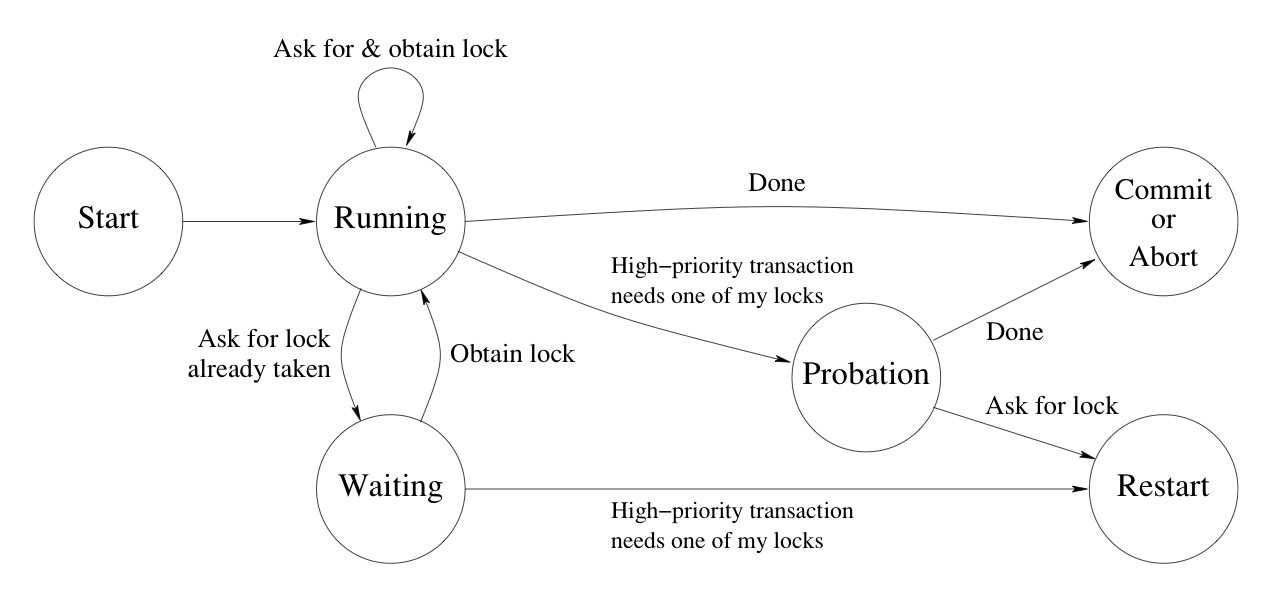
\includegraphics[width=\textwidth]{img/TransDiag}
    \caption{Diagramme d'état de la transaction.}
\end{figure}

\end{document}
